\chapter{Localizing Group Differences over Covariance Trajectories}\label{chap:covtraj}

Important feature identification has been well studied 
in classical statistics, and 
we will start here by adapting those
methods directly.
We will see how marrying
methods from differential geometry
and scan statistics enable
identifying meaningful features
that indicate group differences \textit{over time},
that otherwise would be undetectable
given direct applications of classical
approaches.
%Recent work in graphical models has aimed
%to understand the relationship among
%features when data is collected from
%unique sources, but collected longitudinally.
%Building on Riemannian regression schemes,
%we present a parametric model for fitting
%the progression of variable relationships over time.
We describe theoretical developments
on graphical hypothesis testing,
enabling the identification of 
scientifically important and interesting 
group differences
where classical hypothesis testing
both does not identify meaningful features,
and does not identify unique differences
among known disparate groups of individuals.
The work presented in this chapter was published as a journal article in the Quarterly of Applied Mathematics~\citep{covtraj}.


\section{Introduction}
% intro to graphical models
Multivariate data analysis exploiting the conditional independence structure between features or covariates using 
undirected graphical models is now standard within any data analysis toolbox. 
When the data are multivariate Gaussian, the zeros in the inverse covariance (precision) matrix give conditional independences 
among the variables \cite{lauritzen1996graphical}. Further, if the precision matrix is sparse, we can  
derive dependencies between features when the data are high-dimensional and/or the number of measurements are small. 
The estimation of a graphical model
has been extensively studied
%in statistics and machine learning,
and a rich literature is available describing 
its statistical and algorithmic properties \cite{koller2009probabilistic,jordan1998learning}. 
%Particularly for higher-dimensional settings where the dimension $p$ is allowed to grow, \textit{sparse} estimation of the precision matrix has been well-studied. 
For instance, the so-called \textit{graphical lasso} formulation uses an $\ell_1$-norm penalty on the 
precision matrix and is widely used, and consistency properties 
in the large $p$ regime \cite{cai2011constrained,friedman2008sparse,yuan2010high} are now well understood. 
These formulations have also been extended to various transformations of Gaussian distributions (e.g., non-paranormal)
%, where the 
using rank statistics \cite{liu2009nonparanormal,xue2012regularized,liu2012high}.
%are a consistent estimator of 
%the precision matrix nonzero pattern 

{\em Coupled and Temporal Graphical Models.} 
%In various situations,
Often, data come from two (or more) disparate sources or multiple timepoints.
%, where we seek to estimate 
%a model for each source {\em independently}.
%When the sources share the same variables as well as the
%nd a non-trivial portion 
%of the
%dependency structure, we may decide to pool the data together and estimate a single model in an effort to boost statistical power. However, 
%such an approach invariably masks the heterogeneity in the data-set sources \cite{friston2011functional}. While we want 
%to preserve the common structure, ideally, we also wish to allow for differences among the 
%sources. Consequently, w
Within the last few years, a few proposals have 
described strategies for linking the sparsity patterns of multiple graphical models, e.g., using a fused lasso 
penalty \cite{danaher2014joint} \cite{yang2015fused}. Observe that 
%these ideas assume that the two (or more) models share a similar structure; 
if the data sources correspond to {\em longitudinal} acquisitions, we should expect 
the `structure' to gradually evolve.
%, which is discouraged in direct applications of the above idea. 
%in the case where the model is changing such a construction would not allow for identification of the evolving graph structure. 
Several authors have offered generalizations to address this problem: \cite{zhou2010time} removes the assumption
that each graph is independent and structurally `close'.
Instead, \cite{zhou2010time} can be thought of as a growth model \cite{mcardle2000introduction} defined on these structures: they show how non-identically distributed graphs can be learned over time. 
Recently, the nonparametric procedure in \cite{qiu2015joint} extends these ideas
%via means
to handle multiple sources, each with multiple samples.

The ideas in the literature so far to ``couple'' multiple graphical model estimation modules are mostly nonparametric. 
While such a formulation offers benefits, in many estimation problems, 
parametric models may 
%require fewer samples (better convergence rates) and possibly, 
be more convenient for downstream statistical analysis,
particularly for hypothesis testing \cite{hardle1993comparing,geer2000empirical,roehrig1988conditions}.
Given that the topic of \textit{coupled} graphical models, by itself, is fairly recent, algorithms for {\em parametric estimation} of 
temporal or coupled Gaussian graphical models have not yet been heavily studied. 
%Part of the reason is the difficulty of 
This will involve parameterizing {\em trends} in the highly structured nature of the `response' variable ($\SPD$ matrices). 
%In contrast, w
We find that parametric formulations for manifold-valued data {\em have} been proposed recently \cite{hjkimcvpr2014,cornea2016regression}. %, albeit only in the 
%context of regression models and dictionary learning \cite{xie2013nonlinear}. 
%This result is relevant --- b
Because $\SPD$ matrices form a Riemannian manifold, algorithms
that estimate a parametric model respecting the underlying Riemannian metric are more suitable in many applications as opposed to assuming a Euclidean metric 
on positively or negatively curved spaces \cite{xie2010statistical, fletcher2007riemannian, jayasumanakernel}. We will make a few simple modifications 
(for efficiency purposes) to such algorithms and make use of the estimated parameters for follow-up analysis.

%Unfortunately, their deployment for the $\SPD$ may not always be trivial.

{\em Finding Group-wise Differences.} Assuming that we have a black-box procedure to estimate a parametric model on the $\SPD$ manifold available, 
in many tasks, such an estimation is merely a segue to other analyses designed to answer scientifically meaningful questions. 
For example, we are often interested in asking whether the temporally coupled model estimated using the procedure above differs 
in meaningful ways {\em across} groups induced by a stratification or dichotomous variable (e.g., gender or disease). For instance, is the `slope' in structured response space statistically different 
across education level or body mass index? 
%in if this model differs significantly across two groups.
While the body of work for graphical model estimation is mature, the literature describing hypothesis tests in this
regime \cite{diffnet,belilovsky2015hypothesis}
is sparse at best.
%When considering a single graphical model for each group, \cite{diffnet} propose a framework for two sample testing to discover differences in biological network structures.
%However, to the best of our knowledge no literature exists describing a testing framework for temporal graphical models.
%In this paper we propose a method for evaluating this group difference temporally.
Given that such questions are simpler to answer with alternative schemes (with assumptions on the distributional properties of the data), e.g., structural equation modeling, 
latent growth models and so on \cite{ullman2003structural, mcardle2000introduction}, it seems that 
the unavailability of such tools is limiting the adoption of such ideas in a broader 
cross-section of science. We will seek to address this gap. 

{\em Needles in Temporal Haystacks.} If we temporarily set aside the potential value of a hypothesis test framework for temporal 
trajectories in graphical models, we see that
from an operational viewpoint, such procedures are most effective when a practitioner already has a precise scientific question in mind. In reality, however, 
many data analysis tools are deployed for exploratory analyses to inform an investigator as to which questions to ask. 
Being able to ``localize'' which parts of the model are different across groups over the entire time window can be very valuable. This ability actually 
benefits statistical power as well. Notice that when the stratified groups are not very different 
to begin with, e.g., healthy individuals with presence or absence of a genetic mutation, the
effect sizes are likely to be poor.
Here, while the trends identified on the {\em full} precision matrix may still be different (i.e., there may be a {\em real} signal 
associated with a grouping variable), 
they may not be strong enough to survive significance thresholds. Ideally, what we need here are analogs of the widely used ``scan statistics'' 
for our hypothesis testing formulations for temporal graphical models --- to identify which {\em parts of the signal} are promising. 
Then, even if only a small subset of 
features were different across groups over all time,
%(whereas the complement of this sub-graph were similar, i.e., not different)
we may be able to identify these differential effects efficiently. This benefits Type 2 error, 
provides a practical turnkey product for an experimental scientist, and makes up the key technical results of our work.

%motivation for our selection, cost etc.
%A second key issue we aim to address is that of feature selection. In many medical regimes, the true indicators and dependencies among measured features is unknown. In most analyses feature selection is done manually, generally by the researcher. Structural equation modeling (SEM) in particular is a popular tool which requires the user to choose the features as input for analysis. The first component of SEM requires the \textit{structural model} be specified, that the dependences we wish to determine significant are explicitly stated. Quantitative approaches for feature selection  (cite) have been looked at in machine learning. (elaborate)... In the case of image analysis, scan statistics have been used as a measure to detect regions of high correlation between images (cite what Ming cites). These scan statistics, however, require a selection of a subregion of the image or some strong heuristic to make the problem of searching over all possible window sizes tractable. Recently (ming paper) were able to polynomially bound the number of regions needed to detect highly correlated regions with high probability. Motivated by their work, we attempt to solve a parallel problem. In the case of feature selection among high-dimensional covariance matrices, we aim to identify a subset of features such that the evolution of the correlation matrix is significantly different among two groups.

% ULF GRENANDER
%\begin{mdframed}[hidealllines=true,backgroundcolor=blue!20]
Foundations of our work can be traced back to fundamental developments made by Ulf Grenander in a breadth of fields. Early work with Rosenblatt on the analysis of stochastic processes and time series first brought to light
the fundamental issues of linear modeling in Euclidean space, and demonstrated that in many cases it is necessary to develop methods that take explicit advantage of the inherent structure within data \citep{grenander1957statistical}.
Further pioneering work on the statistical analysis on Lie groups \citep{grenander2008probabilities} provides the basis of the Riemannian statistics mentioned above.
Modern hypothesis testing of these structured, manifold-valued data in image analysis is built upon the his joint work \citep{grenander1998computational}. Here, we marry modern developments in these areas, using recent strides in linear model fitting on manifolds and statistical testing of structured data to develop groupwise testing procedures for longitudinal covariances.
%\end{mdframed}
Concurrent to our work, \cite{su2014statistical,zhang2018rate} have developed similar methods of analyzing the statistical properties of trajectories on the $\SPD(n)$ manifold via the transported square-root vector field. While here we focus on a simple approach to enable localization, these developments can be incorporated into our construction.

Briefly, we provide \textbf{(i)} a simple and efficient parametric procedure for modeling temporally evolving graphical models, \textbf{(ii)} a 
hypothesis test for identifying differences between group-wise estimated models, and \textbf{(iii)} a scan
algorithm to identify {\em those subsets of the features which contribute to the group-wise differences}.
Together, these ideas offer a framework for identifying group-wise differences in temporally coupled graphical models.
%We next cover preliminary concepts, we define our model and present an algorithm, followed by experimental results on both simulated data and neuroimaging data 
%acquired from 
From the experimental perspective, we find scientifically plausible results on 
a unique longitudinally tracked cohort of middle-aged (and young elderly) persons at risk for Alzheimer's disease due to family history, 
but who are otherwise completely cognitively healthy.

The rest of the paper is organized as follows. In Section \ref{sec:mglm} we present an efficient manifold regression procedure for 
modeling covariance trajectories, which serves as a blackbox module in our hypothesis testing framework. 
In Section \ref{sec:hyp-test}, we define our main hypothesis test for group difference analysis over covariance trajectories. 
In Section \ref{sec:loc}, we present a set of technical results describing our localization procedure based on scan statistics, 
as well as derive suitable size corrections to compare across feature subsets. Sections \ref{sec:loceval}, \ref{sec:pipeval}, and \ref{sec:wrap} conclude with
empirical evaluations of our model on synthetic data, various types of demographics/behavior data collected longitudinally 
in the United States from publicly available resources, and finally, our 
analysis on a unique longitudinal dataset (followed since 2001) from a preclinical Alzheimer's disease study involving approximately 1500 individuals.

\section{Characterizing Covariance Trajectories}
\label{sec:mglm}
Our main statistical testing framework, to be described shortly, needs an efficient means for calculating a ``trajectory'' of the feature-by-feature interaction graphs over time
for the given longitudinal data. We now describe a scheme which offers this capability. 
Let $X_t \in \RR^{n_t,p}$ be the design matrix of all $n_t$ samples at time $t$, where $t \in \{1,\ldots,T\}$, and $T$ is the total number of distinct timepoints.
We wish to capture the trends in the relationships between the features as a function of $t$. 
To evaluate the groupwise differences in changes of such interactions, we make use of the fact
that these interactions are commonly captured by correlation or conditional independence, represented by the covariance matrix (with normalized features)
and the precision matrix (the inverse of covariance matrix).

Here we simply use the covariance matrix for each timepoint $t$ to denote the interaction between features, 
$C_t = cov(X_t)$. 
Our goal now is to estimate the parameters of the function, $t \to C_t$. 
We may vectorize the covariance matrix and apply a linear model; its parameters
will give the trajectory in ``vectorized covariance space'' as we scan through $t$. 
But these predictions are {\em not} guaranteed to be valid  $\SPD$ matrices and even if a projection is performed to obtain a covariance estimate, distortions introduced by the process may be significant \citep{fletcher2013geodesic}. 
It is well known that classical vector space models tend to be suboptimal 
in the manifold setting (covariance matrices live on the $\SPD$ manifold)
since they use Euclidean metrics which are defined in the ambient space. For manifold-valued data, Riemannian metrics are shown to be superior in many applications 
\citep{fletcher2007riemannian,banerjee2015nonlinear,jayasumanakernel,tuzel2007human}, 
and are increasingly being deployed in machine learning and statistics. 
We will utilize an appropriate statistical model informed by the manifold-structure of the data and 
then derive a hypothesis 
testing procedure to detect groupwise difference in the changes of interactions between features in longitudinal analysis.
%\subsection{Riemannian Geometry}
% Let $\Mc$ be a \textit{differentiable (smooth) manifold} in arbitrary dimensions. 
%A differentiable manifold $\Mc$ is a topological space that is locally similar to Euclidean space and has a globally defined differential structure. 
% A \textit{Riemannian manifold} is a differentiable manifold $\Mc$ equipped with a smoothly varying inner product.
% The \textit{geodesic curve} is the locally shortest path, analogous to straight lines in $\mathcal{R}^{p}$ --- this geodesic curve will be the object that defines the trajectory of our covariance matrices in $\SPD$ space. 
% Unlike the Euclidean space, note that there may exist multiple geodesic curves between two points on a curved manifold. 
%So, the \textit{geodesic distance} between two points on $\Mc$ is defined as the length of the {\em shortest} geodesic curve connecting two points.
%The geodesic distance helps in measuring the error of our trajectory estimation (analogous to a Frobenius or $\ell_2$ norm based loss in the Euclidean setting).
%The geodesic curve from $y_i$ to $y_j$  is parameterized by a tangent vector in the tangent space anchored at $y_i$ with an exponential map $\EXP(y_i,\cdot ): T_{y_i}\Mc \rightarrow \Mc$. 
%The inverse of the exponential map is the logarithm map, $\LOG(y_i,\cdot):\Mc \rightarrow T_{y_i}\Mc$. These two operations move us back and forth between the manifold and the tangent space. 
%Separate from the above notation, matrix exponential (and logarithm) are simply $\exp(\cdot)$ (and $\log(\cdot)$). 
%Finally, \textit{parallel transport} is a generalized parallel translation on manifolds. Given a differentiable curve $\gamma : \mathcal{I} \rightarrow  \Mc$, where $\mathcal{I}$ is an open interval, 
%the parallel transport of $v_0 \in T_{\gamma(t_0)}\Mc$ along curve $\gamma$ can be interpreted as the parallel translation of $v_0$ on the manifold preserving its length and the angle between $v (t)$ and $\gamma$. 
%The parallel transport of $v$ from $y$ to $y'$ is $\Gamma_{y\rightarrow y'}v$.
\subsection{Riemannian Manifold Regression}
Several regression models for manifold-valued data have been proposed, a majority of 
which are nonparametric \citep{jayasumanakernel,banerjee2015nonlinear}. 
%             , and make use of various distance metrics.
Because of the longitudinal nature of our dataset (and recruitment considerations in neuroimaging studies),
%it is not common for  
sample sizes do not exceed a few hundred participants (typically much smaller). 
%Since in longitudinal neuroimaging study, the number of subjects and the number of their visits is limited. 
We have found that generally, in this regime, parametric methods are better suited and also offer other benefits for downstream applications. 
%Our description below will, therefore, 
Next, we will give a simple parametric model for this problem. 
\begin{figure*}[t]
  \centering
  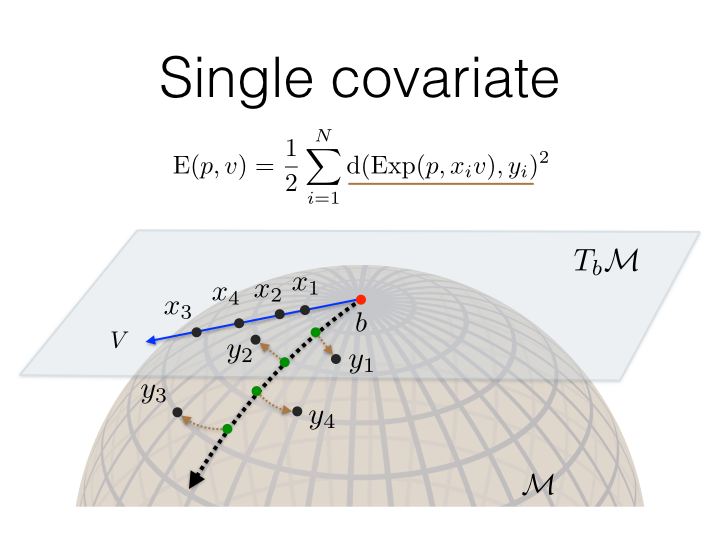
\includegraphics[width=0.49\textwidth,trim={10 40 10 220},clip]{3_covtraj/figs/MGLM1.png}
  %
    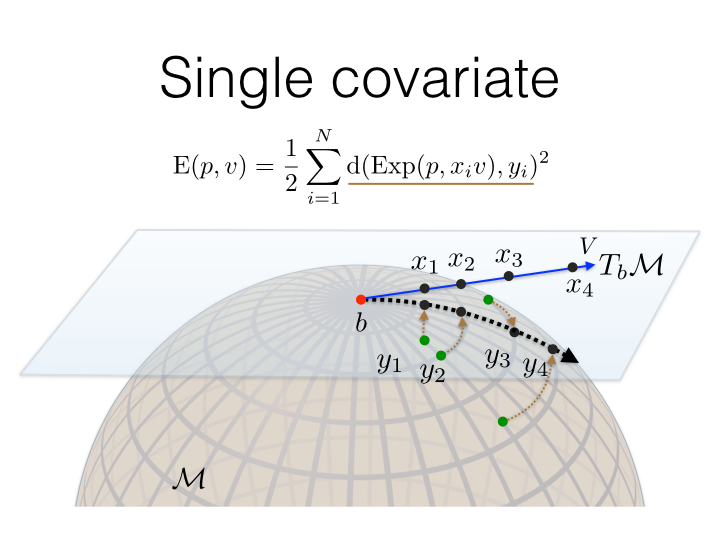
\includegraphics[width=0.49\textwidth,trim={10 40 10 220},clip]{3_covtraj/figs/MGLM2.png}
  \caption[Group-wise comparisons of manifold trajectories]{\label{fig:manifold}Group-wise MMGLM: The left and right figures represent two linear models on the $\SPD(p)$ manifold. Points $x_i$ in the tangent space are our covariate or predictor, and points $y_i$ in the manifold space represent $\SPD(p)$ matrices. In our regression setting, we wish to minimize the error (brown curves) between the estimation and the sample points. Because each linear model has a different base point, the trajectories cannot be directly compared as in the Euclidean setting.}
\end{figure*}
Let $x$ and $y$ be vectors in $\RR^p$ and $\RR^{p'}$ respectively.
\begin{definition} (Standard GLM.) The Euclidean multivariate multilinear model is 
{\begin{equation}
	\begin{split}
	y  = \beta^0 + \beta^{1} x^{1} + \beta^{2} x^{2} + \ldots +\beta^{p} x^{p} + \epsilon
	\end{split}
	\label{eq:generallinear}
	\end{equation}}
where $\beta^0$, $\beta^{i}$ and the error $\epsilon$ are in $\RR^{p}$ and $x = [x^1 \ldots x^p ]^{T}$ are the 
predictor variables.
\end{definition}
Henceforth, we will use the terms \textit{covariate} and \textit{predictor} interchangeably to describe those specific features we wish to control for in our model (e.g., time-points in our experiments).
For manifold-valued data, we adapt the formulation proposed by \cite{hjkimcvpr2014}.
\begin{definition} The Manifold Multivariate General Linear Model (MMGLM) is defined as 
{\begin{equation}
	\begin{split}
	&\min_{b \in \Mc, \forall j, V^j \in T_{b}\Mc} \quad \frac{1}{2} %\sum_{i=1}^{N}d(\EXP(p, {\sum_{j=1}^{n}v^j x_{i}^{j}}),y_i)^2,
	\sum_{i=1}^{N}d(\EXP(b, \textbf{V} x_i),y_i)^2,
	\end{split}
	\label{eq:multigr}
	\end{equation}}
where $\BV x_i \defeq \sum_{j=1}^{n}V^j x_{i}^{j}$, and $d(\cdot, \cdot)$ is the geodesic distance between $\hat{y}_i:=\EXP(b, \textbf{V} x_i)$ and $y_i$. 
\end{definition}
This formulation generalizes \eqref{eq:generallinear}, by replacing the intercept $\beta^0$ and each vector $\beta^j$ for a covariate with a 
base point $b \in \Mc$ and a geodesic basis $V^j \in T_{b}\Mc$ respectively. The geodesic basis $V^j$ at $b$ parameterizes a geodesic curve $\EXP(b,V^jx^j)$.
%for a manifold-valued \textit{dependent} variable is,
%It is clear that in MMGLM each covariate parameterizes a geodesic curve $\EXP(p, v^j x_i^j)$ on $\Mc$. 
Intuitively, this model is a ``generalized'' linear model with the inverse exponential map $\EXP^{-1}$ (or logarithm map $\LOG$) as a 
`link' function \citep{hjkimcvpr2014,cornea2016regression}. When the covariate/predictors are univariate, we will obtain a single geodesic curve, modeled via 
the so-called Geodesic Regression \citep{fletcher2013geodesic}.

\subsection{Efficient Estimation of Trajectories}
\label{sec:effest}
The objective in \eqref{eq:multigr}, can be solved by both gradient descent \citep{fletcher2013geodesic,hjkimcvpr2014} and MCMC methods \citep{cornea2016regression}. 
Unfortunately, these schemes can be expensive, especially when the dimension of the manifold is large. Further, if the algorithm needs to be run a 
large number of times, the computational footprint quickly becomes prohibitive. 
Motivated by these considerations, we use a so-called log-Euclidean approximate algorithm introduced in \cite{hjkimcvpr2014} with some adaptations, which requires mild assumptions on the manifold-valued data. 

Recall that in classical ordinary least squares (OLS), 
the regression curve goes through the mean of covariates and response variables, i.e., $y-\bar{y} = \beta(x-\bar{x})$.
Similarly, we assume that geodesic curves go through the mean of response variables on the manifold. Then, the base point, or intercept, ``$b$'' in \eqref{eq:multigr} can be approximated by the {\em manifold-valued mean of the sample points}, the Karcher mean \citep{karcher1977riemannian}. The propositions derived from \cite{hjkimcvpr2014} lead directly to the following. 
\begin{proposition}
Let $\bar{C}$ be the unique Karcher mean of a sufficiently close set of covariance matrices that lie on a curve $\Omega$. Then $\bar{C} \in \Omega$, and for some tangent vector $V \in T_{\bar{C}}\Mc$ and each $C$, there exists $x \in \mathbb{R}$ such that $C = \EXP(\bar{C},Vx)$. 	
\end{proposition}
This allows us to bypass the fairly involved variational procedure to estimate the base point $b$.

With this approximation of $\hat{b}$ via $\bar{y}$, the remaining variables to optimize are the tangent vectors $\BV$. 
We do so by taking advantage of log-Euclidean schemes. Once the base point is established as the Karcher mean, each data point on the manifold is projected into the tangent space at that point: $\LOG(\bar{y},y)$. These ``centered" points $\tilde{y}$ are now Euclidean, and if the covariates are centered as well ($\tilde{x}$), a closed form solution exists in the standard form of $\BV = \tilde{y}\tilde{x}^\top (\tilde{x}\tilde{x}^\top)^{-1}$ (ordinary least squares). 

In this setting, it is often assumed that two points $y_1,y_2$ have a distance defined as $d(y_1,y_2) := \| \LOG(y_1,y_2) \|_{y_1} \approx \| \LOG(b,y_1)-\LOG(b,y_2) \|_{b}$. However,
on $\SPD$ manifolds with an affine invariant metric, each tangent space has a different inner product varying as a function of the base point $b$, i.e., $\langle  u,v\rangle_b:= \tr (b^{-1/2}ub^{-1}vb^{-1/2})$. This makes comparison of trajectories difficult without moving to tangent bundle formulations. This issue is discussed in some detail in \cite{muralidharan2012sasaki,hong2015group}. However, note that
\begin{remark}
When the base point $b$ is the identity $I$, then the inner product is exactly the Euclidean metric $\langle  u,v\rangle_b:= \tr (b^{-1/2}ub^{-1}vb^{-1/2})=\tr (uv)=\tr (u^Tv)$.
\end{remark}
This follows from the fact that $u$ and $v$ are symmetric matrices on $\SPD(p)$. We take advantage of this property
through \textit{parallel transport}. Specifically, we can bring all of the data to $T_{I}\Mc$ which will allow for a meaningful comparison of two tangent vectors from different base points.
Similar schemes have been used for projection on submanifolds in \cite{xie2010statistical} and other problems \citep{sommer2014optimization}. 
%%More details about optimization on manifolds is available in \cite{}.
%%We now summarize the estimation procedure.
%
With a fast algorithm to compute \eqref{eq:multigr} available, we can now accurately model longitudinal trajectories of covariances matrices.
Our statistical procedure described next simply assumes 
the availability of some suitable scheme to solve the manifold-regression as defined in \eqref{eq:multigr} efficiently and does not
depend on particular properties of the foregoing algorithm. 
%%; other
%%strategies such as those in \cite{cornea2016regression} can also be used directly. 
%%generalize the procedure outlined in \cite{fletcher2013geodesic} to 
%%estimate the tangent vectors $\hat{V}$. 
%%Briefly, 
%
%Let $x^{\wr}_i = x_i -\bar{x}$, and $y^{\wr}_i = \Gamma_{\bar{y}\rightarrow I} \LOG(\bar{y},y_i)$ be the centered $x$ and parallel transported tangent vectors for $y$ in $T_{I}\Mc$ resp.
%For matrix-valued tangent vectors, we treat $y^{\wr}$
%The closed form solution for $\hat{V}$ can now be obtained by $YX^\top(XX^\top)^{-1}$, where 
%$X=[x^{\wr}_1 \cdots x^{\wr}_N]$, $Y=[\text{vec}(y^{\wr}_1) \cdots \text{vec}(y^{\wr}_N)]$ and $\text{vec}(\cdot)$ vectorizes a tangent vector, 
%which is necessary when the tangent vector is matrix-valued, e.g., the symmetric matrix for $\SPD(n)$ manifolds.
%The Karcher mean \cite{karcher1977riemannian} $\bar{y}$ is defined as $\bar{y} = \arg\min_{y \in \Mc} \sum_{i=1}^n w_id(y,y_i)^2 $, where $d(\cdot,\cdot)$ is the geodesic distance.
%When the distance is defined as the length of the logarithmic map $||\LOG_y(y_i)||$, 
%The solution above is a \textit{local} minimum which satisfies $\sum_{i=1}^n \LOG_{\bar{y}} y_i = 0$.
%The global solution to the Karcher mean may not be unique on an arbitrary manifold. For a unique mean to exist, we must make the assumption that all of the data exist within a relatively small neighborhood. Additionally we note that by Propositions 1 and 2 of \cite{hjkimcvpr2014}, the substitution $\hat{p} = \bar{y}$ is not too strong. We assume that our covariance matrices fall on a unique geodesic curve parametrized by a base point and by tangent vectors, and so the conditions which show that the Karcher mean itself lies on this curve are satisfied.
%The last step is to bring the estimated coefficients $\hat{V} \in T_{I}\Mc$ to the tangent space $T_{\bar{y}}\Mc$ by $\Gamma_{I \rightarrow \bar{y}} \hat{V}$.
%Using this procedure, we can efficiently 
%This workflow allows estimating the trajectory of covariance matrices on the $\SPD(n)$ manifold.
% % % % % % % % % % % HYUNWOOs MGLM VARIATONAL STUFF
% This is just in case
%\begin{align}
%min_{p^\wr,\nu} E^{\wr}(p^{\wr},\nu) := \min_{p^{\wr},\nu} \frac{1}{2} \sum_i \| \left(\sum_j \nu^jx_i^j + p^{\wr}\right) - y_i^{\wr}\|^2
%\end{align}
%gradient:
%\begin{align}
%\nabla_{p^{\wr}} E^{\wr} = \sum_i ((\hat{y})i^{\wr} - y_i^{\wr}), \quad \nabla_{\nu^j} E^{\wr} = \sum_i x_i^j (\hat{y}_i^{\wr} - y_i^{\wr})
%\end{align}

\section{Test Statistics for SPD(n) Trajectories}
\label{sec:hyp-test}
With an algorithm to construct a regression model for covariance matrix responses in hand, we can now describe a key
component of our contribution: a test statistic which allows addressing the main question of interest: 
{\em Is the progression/trajectory of covariance matrices (over time) different across two groups?} In the standard two-sample testing problem, a hypothesis test is set up
to check if the parameters of each group are significantly different:
\begin{align}\label{eq:hyptest}
H_0: \theta_1 = \theta_2 \quad vs. \quad H_A: \theta_1 \neq \theta_2
\end{align}
Recall that in a general linear model (GLM), when testing for mean group differences, the test parameters are the regression slopes from a standard GLM fit. 
In our setting, the parameters of interest are the population covariance trajectories estimated from the manifold regression in \eqref{eq:multigr}, see Figure \ref{fig:manifold}. 
While the trajectories and the slopes are related, note that our parameters are estimated {\em on the manifold}. 
Two unique manifold trajectories, when projected as simple multivariate responses in Euclidean space, may not be significantly different under the GLM hypothesis testing framework, as has been observed by \cite{du2014geodesic}. Returning to our longitudinal trajectory formulation, we have the following na\"ive Covariance GLM:
\begin{definition} Let $vec(C_{g,t})$ be the vectorized covariance matrix at timepoint $t$ for group $g \in \{1,2\}$. Then the 
na\"ive Covariance GLM is defined as
\begin{align}\label{eq:euclideanGLM}
vec(C_{g,t}) = \beta_g^{0} + \beta_g t + \epsilon
\end{align}
with the slope $\theta = \beta$ in the hypothesis test in \eqref{eq:hyptest}, and $vec(\cdot)$ is the vectorized form of the input matrix. 
\end{definition}
With this model, hypothesis testing reduces to a simple difference of slopes, which is well-studied in classical statistics literature.
\begin{definition}\citep{seber2003linear} \label{eq:euclideanhyptest}
Let $\Bbeta_1,\Bbeta_2$ be the multivariate slopes calculated from estimating \eqref{eq:euclideanGLM}.
Then an $\alpha$-level hypothesis test rejects the null hypothesis $\Bbeta_1 = \Bbeta_2$ when $L > \chi^2_{p}|_{1-\alpha}$, where
\begin{align}
L = (\hat{\Bbeta}_1 - \hat{\Bbeta}_2)\Sigma^{-1}(\hat{\Bbeta}_1 - \hat{\Bbeta}_2)
\end{align}
\end{definition}
Knowing that the response space is structured, i.e., our covariance matrices lie on the $\SPD$ manifold, we seek a more appropriate test and corresponding test statistic which 
adequately captures this knowledge. 

Observe that we can directly apply the manifold regression in Section \ref{sec:mglm} to solve for a linear model on the manifold. 
That is, we construct the \textit{manifold} GLM as
\begin{definition} Let $C_{g,t}$ be the covariance matrix at timepoint $t$ for group $g \in \{1,2\}$. Then the 
	Longitudinal-Covariance GLM (LCGLM) is defined as
	\begin{align}\label{eq:LCGLM}
		C_{g,t} = \EXP(b_g, \BV_g t)
	\end{align}
	with $b_g$ and $\BV_g$ being the base point and tangent vector respectively, as described in Section \ref{sec:mglm}.
\label{eq:lcglm}
\end{definition}
%Evaluating this model in general turns out to be significantly more involved than the standard vectorized approach. 
But instead of solving $p(p-1)/2$ independent regressions, now we must concurrently solve for the entire manifold-valued response variable.
In this case, we cannot directly compare our trajectories because they lie in {\em different} tangent spaces. To accurately compare two tangent vectors, 
we must parallel transport both vectors to the same tangent space. Once they are both in the same space, we can construct a simple test statistic for the trajectory difference.
\begin{align}
L = \|\Gamma_{b_1 \rightarrow I} \BV_1 - \Gamma_{b_2 \rightarrow I} \BV_2 \|_{I}^2
\label{eq:traj}
\end{align}
Recall that the inner product at the Identity $I$ coincides with the Euclidean metric. This can now be naturally interpreted as a difference of slopes, and together with a standard Euclidean Normal noise assumption yields the following hypothesis test.
\begin{proposition}\label{prop_prodstat}
Assume that $\Gamma_{b \rightarrow I} \BV$ is normally distributed $N(0,I)$. Then the statistic defined in \eqref{eq:traj} follows a $\chi^2_{p}$ distribution with $p$ degrees of freedom, and the threshold test in \eqref{eq:euclideanhyptest} is an $\alpha$-level hypothesis for the covariate trajectory group difference.
\end{proposition}

%\subsection{Test Statistics and Evaluation}
%Recall that F-statistics \cite{} are a textbook procedure to evaluate the two-sample hypothesis test. 
%In our case, however, one subtle issue that needs careful handling is that the null model is not directly nested within the alternative. 
%Specifically, although we use all of the data to fit the null model, the {\em linear models are fit on the manifold} while the {\em data samples are grouped in feature space}. 
%For this reason, we instead use some form of a likelihood ratio statistic instead of the F-statistic. We describe this idea next. 
%
%For each of the three linear models generated (the null and the two separate models among the groups), we calculate the predicted covariance matrix 
%at each timepoint for which we have samples in the feature space.
%\begin{align}
%\hat{\Sigma}_t = \EXP(\hat{p},\hat{V}t)
%\end{align}
%These matrices are then used to calculate the {\em likelihood for each observed sample}. To remove the mean effect, we use the average of the samples $\hat{\mu}_t = \bar{X}_t$ 
%at each timepoint as an estimate. We can now define the likelihood of the progression model $\hat{\Theta} = (\hat{\mu},\hat{\Sigma})$ given the data as
%\begin{align}
%L(\hat{\Theta}|\vec{X}) = L(\hat{\mu},\hat{\Sigma}) = \prod_{t=1}^T \prod_{x: t(x) = t} \frac{1}{\sqrt{2\pi}|\hat{\Sigma}_t|^{p/2}} \exp{\left\{\frac{1}{2}(x - \hat{\mu}_t)^\top \hat{\Sigma}_t (x - \hat{\mu}_t) \right\}}
%\end{align}
%The ratio statistic can then be written in its standard form:
%\begin{equation}
%\lambda(\vec{X}) = \frac{L(\hat{\Theta}|\vec{X})}{L(\hat{\Theta}_1|\vec{X}_{G1})L(\hat{\Theta}_2|\vec{X}_{G2})}
%\end{equation}
%
%In general, the null distribution for a model such as the one above is difficult to characterize, specifically because of the non-nested hypothesis spaces. 
%In place of an exact null distribution, we make use of permutation testing to estimate the null distribution. 
%The statistic of the true group label distribution is then used to calculate a $p$-value for the estimated model. While this is more computationally 
%intensive, this design choice ensures that our results are statistically accurate.

\subsection{Incorporating First-Order Differences}
In many real world situations, first-order information in the data is often valuable in identifying group differences. Restricting 
our analysis to only the second-order interactions, i.e., covariances, may be inefficient (or sub-optimal) when the mean signal difference between groups is large. Our construction easily extends to these cases. Particularly, the \textit{product space} over both means and covariances is in $\mathbb{R}^{p} \times \SPD{(p)}$. 
\begin{remark}
The typical GLM on the first order information is defined in the standard Euclidean space. So, computing the regression in the product space 
$\mathbb{R}^{p} \times \SPD{(p)}$ 
amounts to simply 
computing the regression on the first and second order statistics (mean and covariance) separately.
\end{remark}
The above statement suggests that by applying the manifold regression to the covariances and the standard regression model for the means, 
we are directly solving the product space regression problem, incorporating both first and second order statistics.
However, in these cases, the statistic defined above in \eqref{eq:traj} does {\em not} directly take into account the potential difference in means. 
However, given our Normal noise assumption we can easily invoke the standard Gaussian multivariate likelihood statistic for group differences.
\begin{definition}
Let $\hat{\mu}_t, \hat{\Sigma}_t$ be the estimated mean and covariance from the standard linear model and our manifold-covariance GLM respectively. Then the Gaussian likelihood of our data $X$ is
\begin{align}
P(X|\hat{\mu},\hat{\Sigma}) = \prod_{t=1}^{T}\prod_{i=1}^{n_t} P(X_t | N(\hat{\mu}_t,\hat{\Sigma}_t)),
\end{align}
where $X_t$ is the subset of our data collected at timepoint $t$. Additionally, we can define a standard likelihood ratio test statistic as:
\begin{align}
L_{prod} = \frac{P(X_1|\hat{\mu}_1,\hat{\Sigma}_1)P(X_2|\hat{\mu}_2,\hat{\Sigma}_2)}{P(X_{1,2}|\hat{\mu}_{1,2},\hat{\Sigma}_{1,2})}
\end{align}
\end{definition}
This statistic is again $\chi^2_{p}$-distributed \cite{seber2003linear}, and an $\alpha$-level hypothesis test for group difference analysis 
can be defined in the same way as above. While our manifold regression modeling is focused on the case of centered data (where the mean signal may not be 
significantly different between the groups), we use the product space construction, wherever appropriate, in experimental evaluations.

\section{Localizing Group Differences for SPD(n) Trajectories}
\label{sec:loc}
%One difficulty we have neglected so far is that 

%What we have available at this stage using 
The above procedure provides a precise mechanism to derive a statistic from the group-wise covariance matrix trajectories.
However, when the effect sizes are poor, any scheme operating on 
the trajectories of the {\em full covariance matrix} may still fail to identify group differences (as is the case in our experiments). To improve statistical power, localizing the process of computing the trajectories {\em 
  only to the relevant features} (subset selection) is critical. 
%Additionally, it serves as a discovery tool for exploratory analysis.
%
%
To this end, we consider the following global hypothesis testing problem
\begin{equation*}
H_0: \forall R, \Bbeta_1^R=\Bbeta_2^R \quad vs. \quad H_1: \exists R, \Bbeta_1^R\ne\Bbeta_2^R,
\end{equation*}       
where $\Bbeta$ denotes the slope and $R$ is the \textbf{region of the covariance matrix}
{\em which only includes the relevant features}, see Fig. \ref{fg:ball}.
It turns out that by adapting {\em Scan statistics} \citep{fan2012control, arias2011detection}, we will be able to exclude the effect of irrelevant regions of the covariance 
matrix in the calculated trajectories. 
By extending this concept to graphs, we obtain an algorithm to identify {\em subsets of features} of the covariance matrix which show group differences that 
are otherwise unidentifiable, in a statistically rigorous way. 
%Naively, exponentially many feature subsets $\mathcal{O}(2^p)$ need to be considered when localizing.  Under some mild conditions, extensions of ``scan statistics'' allow computationally tractable localization without compromising type II error.

\subsection{Scan Statistics}
Scan statistics are a valuable tool for structured multiple testing.
%Known in the engineering literature as “moving window analysis”, 
%The main idea is to instantiate o
In its simplest form, we can consider a setting where we place a window (or box) over a region $R$ in an image and calculate 
a local statistic $L_R$, e.g., an average or a response to a convolution filter. 
%a small window over the data, calculating some local statistic (number of events for a
%point pattern, perhaps, or average pixel value for an image) for each window. 
Then, the window can be raster scanned at various locations in the image ($\cR$) and the maximum 
over the set of local statistics is called the scan statistic. 
%The  
%The supremum
%or maximum of these locality statistics is known as the scan statistic, denoted M(X).
%Under
%some specified “homogeneity” null hypothesis H0 on X (Poisson point process, perhaps,
%or Gaussian random field) 
Intuitively, if the image is assumed to be a Gaussian random field, we can set up a null hypothesis using a
critical value and finding a statistically significant signal (i.e., regions) corresponds to comparing 
the local region-wise statistic with the critical value.  
%the approach entails specification of a critical value cα such that
%PH0 [M(X) ≥ cα] = α. If the maximum observed locality statistic is larger than or equal to
%cα, then the inference can be made that there exists a nonhomogeneity—a local region with
%statistically significant signal.
Of course, there is flexibility in terms of specifying properties of the regions as described next. 
 
\begin{definition} Let $\cR$ be the collection of all possible structured regions, and $L_R$ be some statistic over region $R$, a structured subset of $\cR$. The scan statistic is defined as $L^* = \max_{R\in\cR} L_R$.
\end{definition}
Recent results in scan statistics show how \textit{size corrections} can be used to increase detection power in multi-scale analysis with 
nice guarantees \citep{walther2010optimal,wang2016structured}. 
%With size corrections, scan statistics have been shown to be able to detect signal at level that theoretically no other detectors can improve \cite{walther2010optimal,wang2016structured}.
%
To utilize these ideas for our hypothesis test, we must extend scan statistics and these size corrections to a graph setting 
where the graph is induced by a sparse estimation of the precision matrix, e.g., graphical lasso (or any other algorithm of choice) over the features.
%, we can nicely define scan statistics on a graph.
%In order to define scan statistics on a graph, 
%effectively apply these methods, 
To do so, structured regions $R$ and a statistic $L_R$ on each region must be defined on the graph. Intuitively, in our case, 
$L_R$ must capture the ``difference'' in group-wise covariance trajectories. 
As we will describe shortly, it is in the context of this statistic where we utilize the LCGLM \eqref{eq:LCGLM}, which will be invoked at the {\em level of individual regions} $R$, one by one. 
%Since we have 
%In our setting, we can take advantage 
%a natural sparse graph structure which is estimated by graphical lasso in the previous section. 

Let $G:=(\cV,E)$ be a graph over the features (represented in the covariance matrix) with vertex set $\cV$ (to avoid overlap with tangent vectors) and edge set $E$. 
We define the structured region $R \subseteq G$ as a connected subgraph of $G$ corresponding to the 
selection of those vertices as our feature subset (block of the covariance matrix, see Fig. \ref{fg:ball}). 
A natural question is whether such an enumeration is tractable 
if the number of connected subgraphs $\cR$ is exponential. It turns out that if we make a mild assumption on the graph, 
the number of induced regions can be shown to be polynomially bounded. Further, it then naturally provides a {\em size correction}, the analog for a multiple testing adjustment. 

In our motivating application, the group differences we seek to identify will involve a cohesive set of features that will be 
connected to each other, by definition (large changes in covariances indicate dependent features). 
%features in one neighborhood are believed to behave similarly. 
Based on this observation, we assume that the true localized subgraph is a ``ball'' subgraph. 
\begin{definition} A ball subgraph consists of nodes with a given radius $r$ from a particular node (see Fig. \ref{fg:ball}). The collection of ball subgraphs is defined as
\begin{equation}
\cR=\left\{B(v,r):v\in \cV\ {\rm and}\ r\in \NN\right\}
\end{equation}
where the ball subgraph $B(v,r):=\{v^\prime \in \cV:d(v,v^\prime)\le r\}$, and $d(v,v^\prime)$ is the minimum length path connecting $v$ and $v^\prime$.
\end{definition}
%\textbf{Ball subgraph.} The collection of subgraphs of interest can be defined as $\cR=\left\{B(v,r):v\in \mV\ {\rm and}\ r\in \NN\right\}$,
%where the ball subgraph $B(v,r):=\{v^\prime \in V:d(v,v^\prime)\le r\}$, and $d(v,v^\prime)$ is the minimum length path connecting $v$ and $v^\prime$. 
%
With this assumption, it can be verified that we now only need to search a polynomially bounded set of regions.
\begin{remark}
The number of unique ball subgraphs in any graph $G$ is bounded above by $D|\cV|$, where $D$ is the diameter (longest chain) of the graph $G$.
\end{remark}
 On these regions 
(i.e., blocks of covariance matrix), 
we will invoke LCGLM to provide us a statistic $L_R$. This is just the difference in slopes of the calculated manifold regression across groups in \eqref{eq:traj}. 
We will iteratively obtain this statistic for distinct regions $R$ and find subgraphs that differ in their trajectories across groups using a size correction for hypothesis tests.
\begin{figure}
	\begin{center}
		%\scalebox{0.6}
		{
			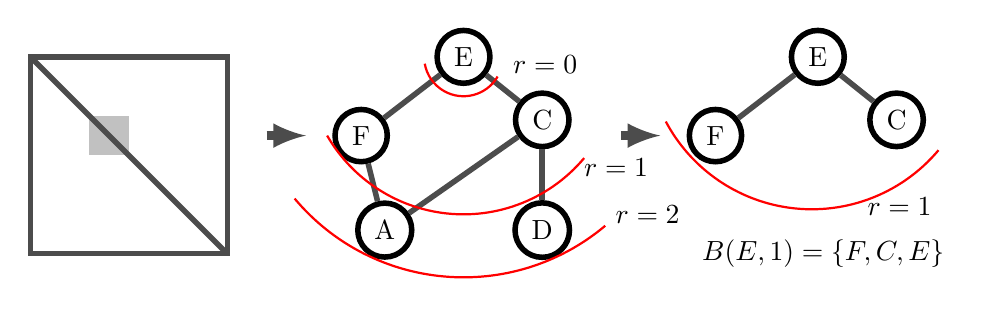
\begin{tikzpicture}
			\path[draw,line width=2pt,black!70!white] (-0.5,-0.5) -- (2,-0.5)--(2,2)--(-0.5,2)--cycle; 
			\fill[black!30!white,fill opacity=0.8] (0.75,0.75) -- (0.75,1.25) -- (0.25,1.25) -- (0.25,0.75) --cycle ; 
			\path[draw,line width=2pt,black!70!white] (-0.5,2)--(2,-0.5);
			
			\draw[-latex,thick,black!70!white,line width=3pt](2.5,1)
			to[out=0,in=180] (3.0,1);
			
			\node[shape=circle,draw=black,line width=2pt] (A) at (4,-0.2) {A};
			\node[shape=circle,draw=black,line width=2pt] (F) at (3.7,1) {F};
			\node[shape=circle,draw=black,line width=2pt] (C) at (6,1.2) {C};
			\node[shape=circle,draw=black,line width=2pt] (D) at (6,-0.2) {D};
			\node[shape=circle,draw=black,line width=2pt] (E) at (5,2) {E};
			\path [draw,line width=2pt,black!70!white] (A) edge node {}  (F);
			\path [draw,line width=2pt,black!70!white] (A) edge node {}  (C);
			\path [draw,line width=2pt,black!70!white] (E) edge node {}  (F);
			\path [draw,line width=2pt,black!70!white] (E) edge node {}  (C);
			\path [draw,line width=2pt,black!70!white] (C) edge node {}  (D);
			
			\draw[-latex,thick,black!70!white,line width=3pt](7.0,1)
			to[out=0,in=180] (7.5,1);
			
			\node[shape=circle,draw=black,line width=2pt] (B2) at (8.2,1) {F};
			\node[shape=circle,draw=black,line width=2pt] (C2) at (10.5,1.2) {C};
			\node[shape=circle,draw=black,line width=2pt] (E2) at (9.5,2) {E};
			\path [draw,line width=2pt,black!70!white] (E2) edge node {}  (B2);
			\path [draw,line width=2pt,black!70!white] (E2) edge node {}  (C2);
			
			\draw[thick,red] ([shift=(-40:2)]9.5,2.1) arc (-40:-152:2.1);
			\draw[thick,red] ([shift=(-40:2)]5,2) arc (-40:-150:2);
			\draw[thick,red] ([shift=(-30:0.5)]5,2) arc (-30:-170:0.5);
			\draw[thick,red] ([shift=(-50:2.8)]5,2) arc (-50:-140:2.8);
			
			\draw[thick,black](5.5,1.9)node[right]{$r=0$};
			\draw[thick,black](6.4,0.6)node[right]{$r=1$};
			\draw[thick,black](6.8,0)node[right]{$r=2$};
			%         \draw[thick,black](8.7,0.8)node[right]{$B(E,1)$};
			\draw[thick,black](10,0.1)node[right]{$r=1$};
			%\draw[thick,black](0.4,-1.3)node[right]{$(a)$};
			%\draw[thick,black](4.75,-1.3)node[right]{$(b)$};
			%\draw[thick,black](9.15,-1.3)node[right]{$(c)$};
			\draw[thick,black](7.9,-0.5)node[right]{$B(E,1)=\{F,C,E\}$};
			
			\end{tikzpicture}
		}
	\end{center}
	\caption{\label{fg:ball} (left) A region of the sparse precision matrix, (center) The corresponding subgraph of that region, along with balls of varying radius from the root node $E$, (right) The ball subgraph constructed with $r = 1$.  These subgraphs with bounded radius act as the 
		structured regions on which scan statistics can be applied.}
\end{figure}
%To measure the change of dependence relationship between features, 
%we first fit a linear model for each element on covariance matrices over time for each group, i.e.,  $\beta_{g,ij} = \arg\min_{\alpha,\beta} \sum_{k=1}^T \|S_{k,g,ij} - \alpha - t_k\beta\|^2$, where $g$ is a group index $\{1,2\}$.
%the regression coefficient fit to the $i,j$-th position of the covariance matrices for both groups, i.e., $\beta_{g,ij} = \arg\min_{\alpha,\beta} \sum_{k=1}^T \|S_{k,g,ij} - \alpha - t_k\beta\|^2$. We call $B_g:=\beta_{g,ij}$ as a slop matrix.
%Now, we define a measurement, denoted by $X_e=|\beta_{1,ij} - \beta_{2,ij}|$, on each edge $e=(i,j)\in E$, indicating the correlation slope difference between feature $i$ and $j$.  To investigate the group effect within a subgraph $R$, it's straightforward to define a simple statistic as
%% \begin{align}
%% L_R = {\sum_{(i,j)\in E(R)}|\beta_{1,ij} - \beta_{2,ij}|\over \sqrt{|E(R)|}}
%% \end{align}
%where $E(R)$ represents all edges induced by subgraph $R$ and $|E(R)|$ is the number of edges in $E(R)$.
%To keep the variance of $L_R$ the same, we use $\sqrt{|E(R)|}$ instead of $|E(R)|$ in denominator of  $L_R$.
%Defined in this manner the calculation of this statistic is simple; we compute $L_{\cR}$ over all features, and then $L_R$ is simply the submatrix of $L_{\cR}$ indexed by the features $i,j \in R$.

Let us revisit the standard linear model setting and assume that 
our slopes $\Bbeta_g^R$ correspond to the subset of slopes from features in $R$, and $\hat{\Bbeta}_g^R$ is an estimate of that slope. In this case, we have the following  statistic (see e.g. \cite{seber2003linear}),
\begin{align}
(\hat{\Bbeta}_1^R - \hat{\Bbeta}_2^R)\Sigma_R^{-1}(\hat{\Bbeta}_1^R - \hat{\Bbeta}_2^R) \sim \chi_{|E(R)|}^2,
\end{align}
where $\Sigma_R^{-1}$ is the covariance matrix of $\hat{\Bbeta_1^R} - \hat{\Bbeta_2^R}$, and $E(R)$ denotes the number of edges among vertices in the subgraph $R$. With a normal noise assumption, this covariance will 
be identity and the statistic would simply be the $\ell_2$-norm difference as in the classical analysis. 
To make the statistics comparable across {\em different sizes}, we use the standardized version of a $\chi_{|E(R)|}^2$ distribution,
{\small\begin{align}\label{eq:LRstat}
L_R = \frac{(\hat{\Bbeta}_1^R - \hat{\Bbeta}_2^R)\Sigma_R^{-1}(\hat{\Bbeta}_1^R - \hat{\Bbeta}_2^R) - E(R) }{ \sqrt{E(R)} }.
\end{align}}
We can extend this analysis to our manifold setting.
\begin{definition}
For a given structured region $R$, the region-based LCGLM is written as
{ \begin{equation}
%\begin{split}
(b_g^R,\BV_g^R) = \arg\min_{(b^R,\BV^R) \in T\Mc^R} 
	\EE \left[ d(\EXP(b^R, \BV^R t_g),C_g^R)^2\right]
%\end{split}
\end{equation}}
where $C_g^R$ is the covariance matrix subblock defined by features included in $R$ for group $g$ ($t_g$ is our univariate predictor, i.e., time).
\end{definition}
\todo{ch3: fig: pt+stat pipeline}
To compare the group trajectories, we first parallel transport each tangent vector to the identity as described in \S\ref{sec:mglm} and then compute the statistic in \eqref{eq:traj} given as $\|\Gamma_{b_1^R \rightarrow I} \BV_1^R - \Gamma_{b_2^R \rightarrow I} \BV_2^R \|_{I}^2$.
In the case of the product space construction, we apply the test in \eqref{prop_prodstat} to the data subset corresponding to the features 
in region $R$, with the same correction as in \eqref{eq:LRstat}.

\paragraph{Summary.} We now have a region-based statistic for the manifold regression setting that is approximately normally distributed $N(0,1)$, allowing effective comparison across differently-sized regions.

%\iffalse
%{ \color{red}
%Now, given a structured region $R$, we can define $L_R$ using our statistic from Section \ref{sec:hyp-test}. The MMGLM defined for region $R$ can be written as
%\begin{equation*}
%\begin{split}
%(b_g^R,\BV_g^R) = \argmin_{(b^R,\BV^R) \in T\Mc^R} 
%	\EE \left[ d(\EXP(b^R, \BV^R t_g),C_g^R)^2\right]
%\end{split}
%\end{equation*}
%where $C_g^R$ is the subblock of the covariance matrix defined by the features included in $R$ for group $g$ and $t_g$ is our univariate predictor, time. With this estimate of the mean and tangent vector for both groups, the statistic is as in \eqref{eq:traj}, with a slight adjustment. If we normalize by the covariance of our estimate, this difference of slopes can be naturally interpreted as $\chi^2$ distributed with $E(R)$ degrees of freedom.{\color{blue}(If we don't introduce linear model and normal assumption, we can't say it follows the chi square distribution!!! We have to introduce linear model theory and say the manifold can borrow idea from there, otherwise the claim is wrong. We also need to distinguish the true value $\Bbeta^R$ and estimator $\hat{\Bbeta}^R$)} Let the vectorized ``slopes" for groups 1 and 2 be $\Bbeta_g^R = vec(\Gamma_{b_g^R \rightarrow I} \BV_g^R)$. {\color{blue}In linear model (see, e.g. \cite{seber2003linear})},  
%\begin{align}
%(\hat{\Bbeta}_1^R - \hat{\Bbeta}_2^R)\Sigma_R^{-1}(\hat{\Bbeta}_1^R - \hat{\Bbeta}_2^R) \sim \chi_{|R|}^2
%\end{align}
%{\color{blue}Here $\Sigma_R$ is the covariance matrix of $\hat{\Bbeta}_1^R - \hat{\Bbeta}_2^R$. To make statistics comparable across different sizes, we use the standardized version} of a $\chi_{|R|}^2$ distribution,
%{\begin{align}
%L_R = \frac{(\hat{\Bbeta}_1^R - \hat{\Bbeta}_2^R)\Sigma_R^{-1}(\hat{\Bbeta}_1^R - \hat{\Bbeta}_2^R) - E(R) }{ \sqrt{E(R)} }
%\end{align}
%}
%We have a region-based statistic that is approximately normally distributed $N(0,1)$.
%}
%\fi
\subsection{Size Correction}
%To improve detection power, 
A final unresolved yet important issue is that we must correct $L_R$ based on the number of edges $E(R)$ in $R$.
%Following the ideas of \cite{wang2016structured}, 
This has a direct consequence on detection power.
Observe that the normalization for size correction should be determined by the null distribution of $L_R$, i.e., 
when there is no slope difference in the trajectories between groups.
In order to derive a correction, we need to characterize the behavior of scan statistics within roughly similar regions, $\max_{R\in \cR(A)}L_R$, 
where $\cR(A)$ is the collection of region $R$s with similar size as $E(R)$,
\begin{align}
\cR(A)=\{R\in \cR:A/2<|E(R)|\le A\}.
\end{align}
Clearly, the behavior of $\max_{R\in \cR(A)}L_R$ depends on the ``complexity'' of $\cR(A)$. 
A clear understanding of how similar subgraphs relate to each other leads directly to a correction tied to their relative sizes.

To investigate the complexity of $\cR(A)$, we define the following quantities.
\begin{definition} The distance between subgraphs $R_1$ and $R_2$ can be given as
{\begin{align}
d(R_1,R_2)=1-\frac{|E(R_1)\cap E(R_2)|}{ \sqrt{|E(R_1)||E(R_2)|}}
\end{align}}
\end{definition}
\begin{definition}
Let the $\epsilon$-covering number of $\cR(A)$, denoted by $N(A,\epsilon)$, be the smallest integer such that there
is a subset $\cR_{approx}(A,\epsilon)$ of $\cR$ such that
{\begin{align}
\sup_{R_{1}\in\cR(A)}\inf_{R_{2}\in \cR_{approx}(A,\epsilon)}d(R_{1},R_{2})\le \epsilon
\end{align}}
where $|\cR_{approx}(A,\epsilon)|=N(A,\epsilon)$.
\end{definition}
We can verify that all regions in $\cR(A)$
can be approximated by regions in $\cR_{approx}(A)$ with reasonably small error.
From the definitions, notice that the complexity of $\cR(A)$ is reflected by $N(A,\epsilon)$.
If $N(A,\epsilon)$ is nicely bounded (as is the case here), scan statistics can be calculated very efficiently 
(Lemma \ref{lm:entropy}). 
%, as presented 
%shortly in Lemma \ref{lm:entropy}.
%For more details and intuition, please refer to \cite{wang2016structured}.

Before stating this result, we make a mild assumption on our graph. 
For any ball subgraph, the edges around its center are not too sparse, compared to the edges 
in the outer region of the ball subgraph, i.e., hard on the inside, soft on the outside. This yields, 
\begin{assumption}(Avocado) There exist constants $S$ and $H$ such that, for any $r/2 \leq r' \leq r$ and $v \in \cV$,
{\begin{align}\label{eq:lightskirt}
\frac{|E(B(v,r'))|}{|E(B(v,r))|} \geq H\left(1 - \frac{|E(B(v,r-r'))|}{|E(B(v,r))|}\right)^S.
\end{align}}
\end{assumption}
We see that this assumption holds for many classes of graphs:
a ring graph satisfies this condition when $H=1$ and $S=1$ and the 2-D lattice satisfies this condition when $H=1/4$ and $S=2$ (see Fig. \ref{fg:avocado}). 
\begin{figure}
	\begin{center}
		\scalebox{0.8}
		{
			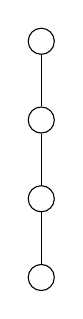
\begin{tikzpicture}
			\tikzstyle{vertex}=[circle,draw,minimum size=0.2cm]
			\tikzstyle{every node}=[vertex]
			
			\node (A) { };
			\node (B) [below of = A] { };
			\node (C) [below of = B] { };
			\node (D) [below of = C] { };
			\draw (A) -- (B);
			\draw (B) -- (C);
			\draw (C) -- (D);
			
			
			\end{tikzpicture}
			\hspace{0.2cm}
			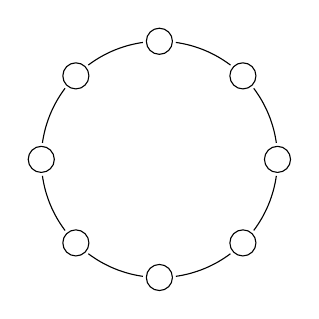
\begin{tikzpicture}
			\def \n {8}
			\def \radius {1.5cm}
			\def \margin {8} % margin in angles, depends on the radius
			
			\foreach \s in {1,...,\n}
			{
				\node[draw, circle] at ({360/\n * (\s - 1)}:\radius) { };
				\draw[-, >=latex] ({360/\n * (\s - 1)+\margin}:\radius) 
				arc ({360/\n * (\s - 1)+\margin}:{360/\n * (\s)-\margin}:\radius);
			}
			\end{tikzpicture}
			\hspace{0.2cm}
			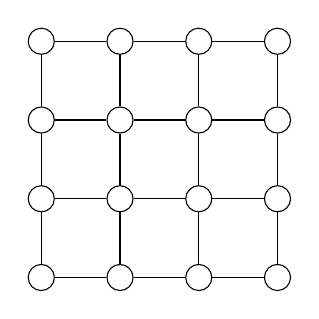
\begin{tikzpicture}%[circle, draw, minimum size=1cm, every node=[vertex]]
			\tikzstyle{vertex}=[circle,draw,minimum size=0.2cm]
			\tikzstyle{every node}=[vertex]
			\foreach \x in {1,2,3,4}
			{
				\foreach \y in {1,2,3,4}
				{
					\node (\x \y) at (\x,\y) { };
					\ifnum\y>1
					\pgfmathparse{int(\y-1)}  
					\draw  (\x \y)  -- (\x \pgfmathresult);
					\fi
					\ifnum\x>1
					\pgfmathparse{int(\x-1)}                
					\draw (\x \y) -- (\pgfmathresult \y);
					\fi 
				}
			}   
			\end{tikzpicture}
			\hspace{1cm}
			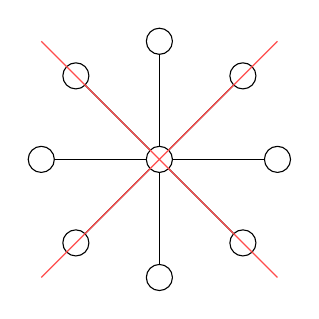
\begin{tikzpicture}
			\def \n {8}
			\def \radius {1.5cm}
			
			\node[draw, circle] (ss) at ({0}:0) { };
			
			\foreach \s in {1,...,\n}
			{
				\node[draw, circle] (\s) at ({360/\n * (\s - 1)}:\radius) { };
				\path (ss) edge [] node { } (\s);
			}
			\path[draw,line width=0.5pt,red!70!white] (-1.5,1.5)--(1.5,-1.5);
			\path[draw,line width=0.5pt,red!70!white] (-1.5,-1.5)--(1.5,1.5);
			\end{tikzpicture}
		}
	\end{center}
	\caption{\label{fg:avocado} (Left) Chain, ring and 2D lattice graphs that satisfy the Avocado Assumption. (Right) Star graph that does not satisfy the property: from the center node the graph is ``too dense on the outside."}
\end{figure}
With this assumption, we have the following result for the $\epsilon$-covering number $N(A,\epsilon)$.
\begin{lemma}
	\label{lm:entropy}
        Let $|E|$ be the total number of edges in $G$. If (\ref{eq:lightskirt}) holds and $A$ is given, 
        then, for a constant $C_{H,S}$ which only depends on $H$ and $S$ in (\ref{eq:lightskirt}),
	{\begin{equation}
	    \label{eq:entropy}
	    N(A,\epsilon)\le C_{H,S}\frac{|E|}{ A}\left(\frac{1}{ \epsilon}\right)^{S+1}.
	\end{equation}}
\end{lemma}
The proof of this result follows from our ball-subgraph construction and our Avocado assumption and is provided in the Appendix.

Intuitively, this result upper bounds the number of graphs that are necessary to search over to completely exhaust the search space of subgraphs. With this result, we can now construct a suitable size correction. 
Following the work of \cite{walther2010optimal} and \cite{wang2016structured}, we can increase the power of our test by using the following statistic:
% when there's no correlation slope difference across groups. 
%To simplify the analysis, we assume null distribution of each $L_R$ follows normal distribution with mean $0$ and variance $1$ at this moment. This assumption generally holds when tangent normal noise assumption.
%And we also assume $L_{R_1}-L_{R_2}$ follows normal distribution with mean $0$ and variance $C'd(R_1,R_2)$ for some constant $C'$. 
%The intuition behind this assumption is that $L_{R_1}$ should behave very similar with $L_{R_2}$ when $R_1$ and $R_2$ has large overlapping region(i.e. $d(R_1,R_2)$ is small).
%Although this assumption does not always hold, this can guide us to obtain the suitable form of size correction.
%With these assumptions, we can actually obtain following theorem:
% \begin{theorem}
% If $X_e$ follows independent normal distribution $N(0,1)$ and (\ref{eq:entropy}) holds, then, for all $t>1$,
% \begin{align*}
% \PP\left(\max_{R\in \cR(A)}L_R> \sqrt{2\log{|E|\over A}}+t\right)\le C_1\exp\left(-C_2t^2\right) 
% \end{align*}
% for some constant $C_1$ and $C_2$.
% \end{theorem}
%Motivated by this result, the suitable way to do size correction is to subtract $\sqrt{2\log{|E|/|E(R)|}}$ from each $L_R$. 
%Therefore, we propose the following this size corrected scan statistic:
{\begin{align} \label{eq:scanstat}
T^\ast=\max_{R\in\cR}\left(L_R-2\sqrt{\log\frac{|E|}{ |E(R)|}}\right).
\end{align}}
%This result requires that the measures over each region that define $L_R$ are defined on each edge $E(R)$. In our particular construction, the statistic $L_R$ is defined as a function a complete measure of the difference of the tangent vectors. Therefore, we can define our \textit{manifold-valued size corrected scan statistic} as:
%{\begin{align} \label{eq:manscanstat}
%T^\ast=\max_{R\in\cR}\left(L_R-\sqrt{2\log\frac{|\text{dim}(\Mc)|}{ |\text{dim}(\Mc^R)|}}\right).
%\end{align}}
The significance of this size correction is that we now have \textit{a single critical value for each candidate subgraph, regardless of the subgraph size}. Our final test is defined as $\mathbb{I}[T^* > q_\alpha]$, where $q_\alpha$ is the $\alpha$-level quantile of $T^*$ under the null hypothesis (that no region is truly significant across groups). By construction, we can control the type 1 error at a specified $\alpha$-level.

Under the alternative hypothesis of this framework, it is important to note that in many cases,
large subgraphs that subsume smaller significant graphs may also have large test statistics, and our hypothesis test only indicates the existence of {\em some} significant region. To identify or localize the smaller subsets, we follow the procedure from \cite{jeng2010optimal}, by beginning with the subgraph with the largest test statistic and iteratively removing overlapping subsets from the total set of subgraphs. This requires testing each regional/local statistic, $(L_R - 2\sqrt{\log(|E|/|E(R)|)})$ against $q_\alpha$. Under this procedure, we can control the weak family-wise error rate (wFWER) if we view our problem via the lens of multiple testing. The weak FWER is the probability of false discovery under the null hypothesis. To see that this is inherently controlled, note
\begin{align}
\mathbb{P}(FN \geq 1|H_0) = \mathbb{P}(T^* > q_\alpha|H_0) \leq \alpha, 
\end{align}
where $FN$ is the number of false discoveries under the null hypothesis. With this correction at the group difference level, we completely avoid any multiple comparisons issues that would arise in the case of a test for each subgraph.
%
In addition to controlling the false positive rate, we have the following guarantee on {\em identifying truly significant regions} under the normal noise assumption.
\begin{theorem}
If \eqref{eq:lightskirt} holds and the number of edges in the candidate subgraph is larger than $\log^2 |E|$, i.e.,
\begin{equation}
\label{eq:setsize}
|E(R)|\gg \log^2 |E|\qquad \forall\ R\in\cR,
\end{equation}
then the critical value $q_\alpha$ satisfies
\begin{equation}
\label{eq:criticalvl}
q_\alpha=O(1).
\end{equation}
Moreover, as $|E|\to \infty$, if a subgraph $R_0$ obeys 
\begin{equation}
\label{eq:sigcond}
\frac{(\Bbeta_1^{R_0}-\Bbeta_2^{R_0})^T\Sigma_{R_0}^{-1}(\Bbeta_1^{R_0}-\Bbeta_2^{R_0})}{\sqrt{|E({R_0})|}}\gg 2\sqrt{\log\frac{|E|}{|E({R_0})|}},
\end{equation}
then as $|E|\to \infty$,
\begin{equation}
\label{eq:power}
\PP\left(L_{R_0}-2\sqrt{\log\frac{|E|}{|E({R_0})|}}>q_\alpha\right)\to 1.
\end{equation}
\label{lm:mainthm}
\end{theorem}
The full proof of this result follows a generic chaining argument (see, e.g. \cite{talagrand2006generic}) along with application of 
concentration inequalities and union bounds, and can be found in the Appendix. \todo{ch3: FWER proof appendix reference}

\paragraph{Summary.} At a high level, this result directly characterizes the behavior of $T^*$ under the null hypothesis $H_0$ and 
the alternative hypothesis $H_1$, respectively. 
We see that \eqref{eq:criticalvl} implies that $T^*$ can roughly be seen as a constant under the null hypothesis, 
and under the alternative hypothesis when \eqref{eq:sigcond} is satisfied, the test based on $T^*$ is consistent, see \eqref{eq:power}. 

\subsection{Workflow for conducting hypothesis tests on temporal trends of graphs}
\todo{ch3: fig: from presentation, full workflow}
%{\color{red} maybe refer to the video again?}{\color{blue} I think a flow chart of how the whole algorithm work may be helpful. Otherwise, it's difficult for audiences to get the idea if we only mention the test statistics and Jeng's paper.}
With these guarantees, our full workflow is as follows. First, we use an oracle procedure to generate a graph over our features 
that roughly captures the conditional independences. Any procedure that provides a conditional independence graph is sufficient. 
Next, for each ball subgraph over this graph, we compute the Longitudinal-Covariance GLM over these features for both groups, and compute the statistics outlined in Section \ref{sec:hyp-test}. We then compute the size-corrected statistic, and compare against the single critical value. For all regions that pass this threshold, we apply the procedure from \cite{jeng2010optimal}. This workflow shows how to conduct hypothesis tests on temporal trends of large covariance matrices, with improved 
power and bounded Type 1 error. Additional implementation details can be found in the Appendix.

\section{Localization Evaluation: Trends of Tobacco Usage Across Gender}
\label{sec:loceval}
We begin our empirical analysis of the model by first applying the subgraph localization procedure by itself (standalone), separate from our manifold regression scheme. In this case, our statistic is derived from {\em only} Generalized Linear Models (GLM) constructions, where the $\hat{\Bbeta}_g^R$ in equation \eqref{eq:LRstat} is the slope estimated from fitting standard first order linear models. Identifying the differentially varying subgraphs across groups in this way is similar to a simpler version of the planted clique identification problem \citep{arora2009computational}, where the clique we are trying to identify corresponds to those nodes whose slopes vary significantly across groups.
\begin{figure}
	\begin{center}
		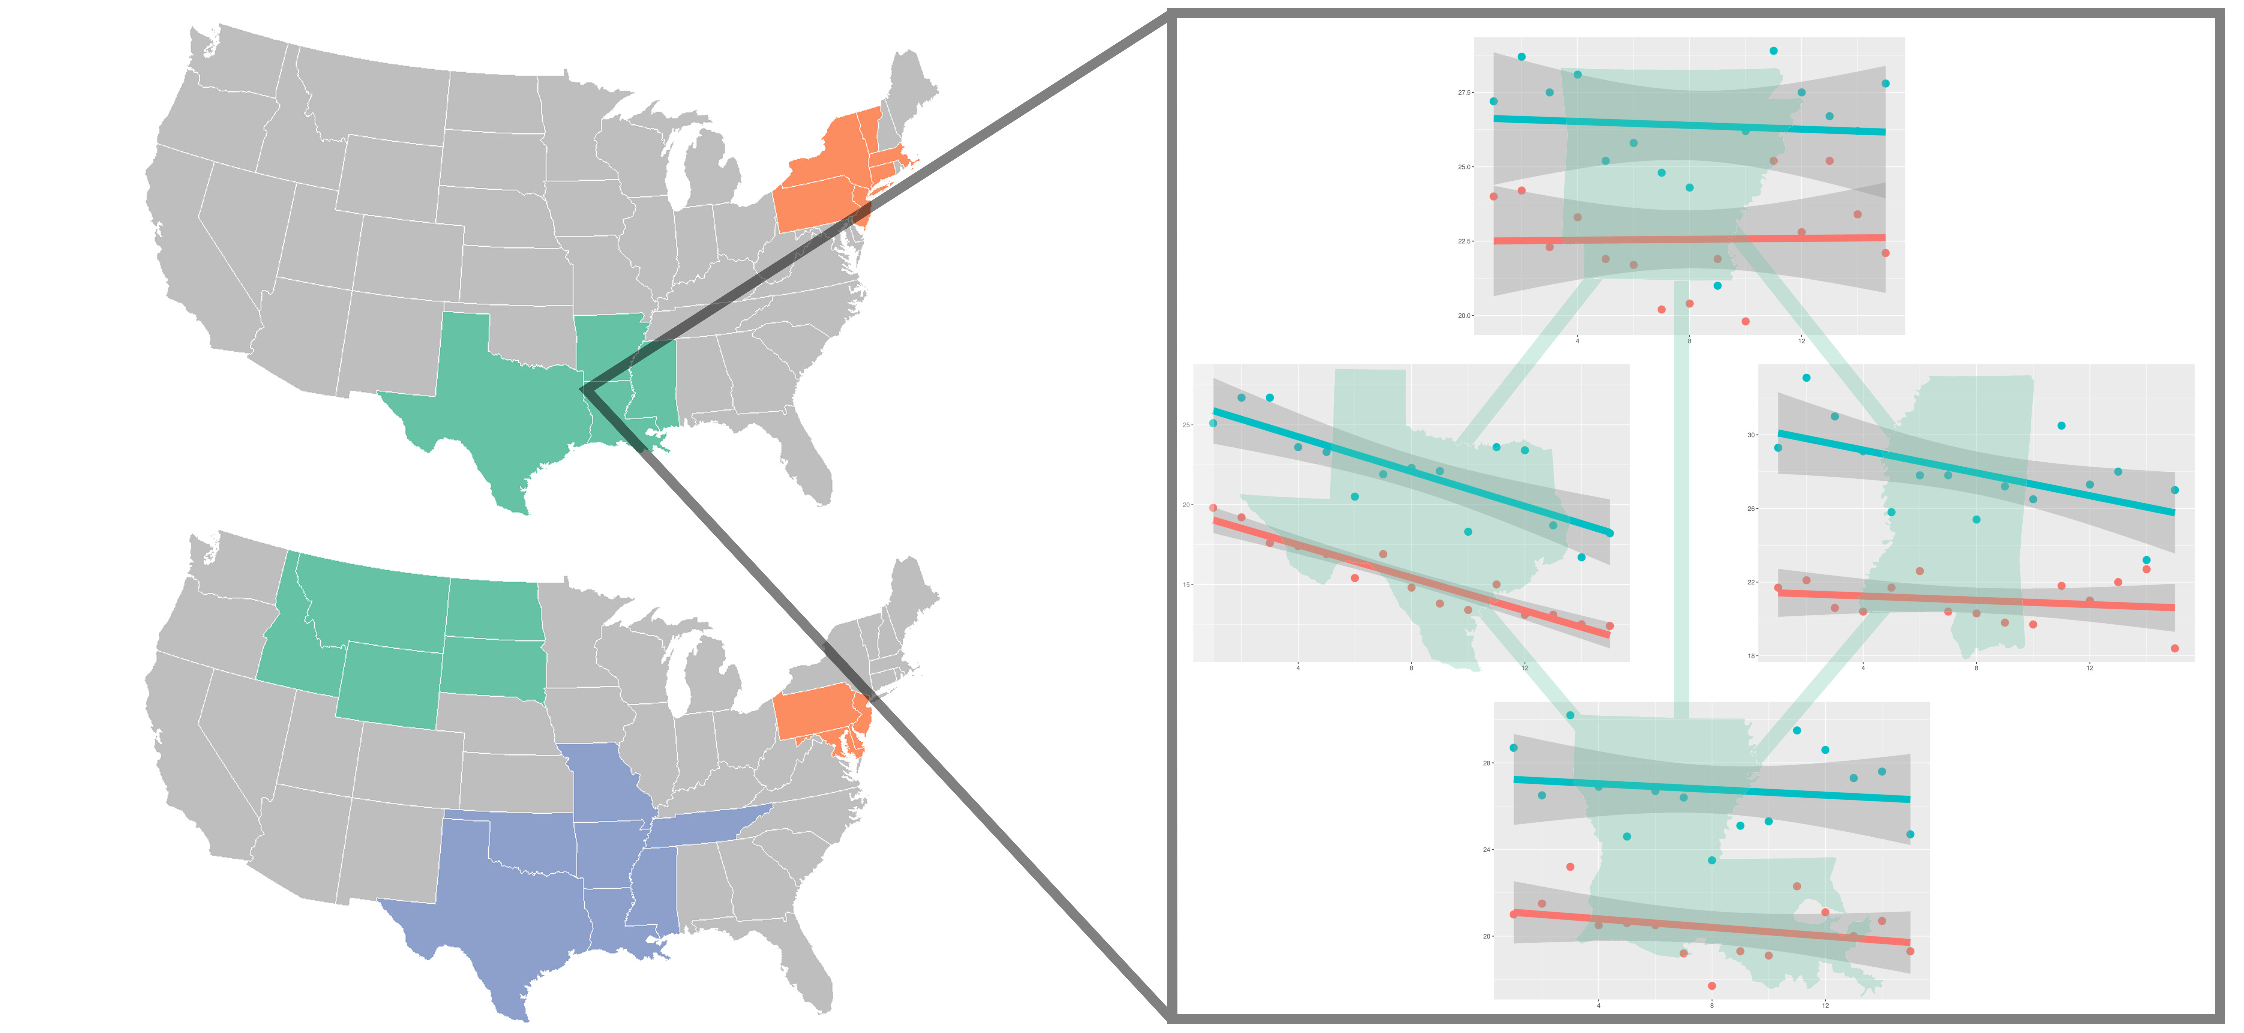
\includegraphics[trim={0cm 0cm 0cm 0cm}, clip, width=0.9\textwidth]{3_covtraj/figs/tobacco_zoom.pdf}
	\end{center}
	\caption[Tobacco use relationships via covariance trajectory analysis]{(left,top) States identified as having significantly different time-varying tobacco usage across gender from 2001 to 2015. (left,bottom) States identified as having significantly different time-varying heavy drinking use across gender from 2010 to 2015. (right) Linear regressions over tobacco usage fitted to the four states defined by the ball subgraph centered at Louisiana. Best viewed in color.}
	\label{fig:tobalc}
\end{figure}

{\em Data.} The Center for Disease Control (CDC) provides extensive statistics regarding tobacco and alcohol usage across the US. This data has been collected systematically for the last few decades and is publicly available (includes demographic information and gender). As a simple application of our 
proposed framework, 
we may pose the following question: which ``sub-groups'' of states tend to evolve differently in their correlation (pertaining to tobacco/alcohol usage) over time? 
Our framework extends easily to answer this question. In this setup, the oracle graph is simply the adjacency graph of the continental
US which will be used directly in our scanning procedure.
For this dataset, we have direct observations of node measures: the percentage of males and females who 
reported smoking or drinking heavily in each state. Using 
gender as the group, 
we fit standard linear models for each candidate subgraph, and compute the difference of gender-wise 
slopes statistic as described above. 
In Figure \ref{fig:tobalc}, we see the regions identified using our method, and interpret some of the tobacco usage findings here.

In the northeast, we see that women have reduced their tobacco usage at a significantly faster rate than men compared to the rest of the country. 
%http://www.who.int/bulletin/archives/78(7)891.pdf
We suspect that this may be at least partly tied to the development of women's cigarette brands in the late 1960s and 1970s 
followed by subsequent aggressive public policy campaigns in the 1990s and 2000s to highlight health risks beyond 
pulmonary or cardiovascular diseases for women (e.g., infertility, reduced bone-density in post-menopausal women). We also see that 
state-wide indoor smoking bans were put in place in the Northeast 
%\href{https://en.wikipedia.org/wiki/List_of_smoking_bans_in_the_United_States}{(2003/2004)} 
ahead of many other states in the union.  
In the South, the trends among men and women also seems to differ significantly. (see Figure \ref{fig:tobalc}). 
Apart from health factors, the group-wise differences in the group-wise trends may also be explained by 
a few reasons identified in a study in 2007 \citep{HEC:HEC1223} which found that as the state sales tax on cigarettes changed (increased), 
women were significantly more price elastic than men. Between 2006 and 2008, the cigarette tax increased dramatically for all of the 4 states identified \textit{except for Louisiana}, whose tax rate has remained constant. Additionally, while Arkansas did increase their cigarette tax in 2009, they did \textit{not increase taxes in locations near borders shared with higher taxing states}. These intricate relationships among states lend credibility to the fact that our scan statistics framework is indeed identifying interesting sub-regions, and suggests that the full covariance-trajectory pipeline may be more appropriate if effects beyond the means are relevant within an analysis. 

%With heavy alcohol usage in the South, West, and Northeast, the prevalence of heavy drinking seems to be declining faster in men. 
%

\section{Pipeline Evaluation on Simulations}
\label{sec:pipeval}
We next evaluate the ability of our entire analysis 
pipeline to identify group differences across temporally evolving \textit{covariance} trajectories. 
In many existing analyses, the effect of the mean differences may be stronger than the effect of the interaction matrix. 
However, in cases where the {\em mean signal is weak}, we expect that the covariance effect will be important. 
To evaluate our model in this regime, we perform a set of simulation studies and also analyze a publicly available longitudinal dataset.

\paragraph{Simulations.} We randomly generate SPD matrices from a `path' of 4 discrete points along the manifold, and use these data 
as population 
covariance matrices to generate 0-mean sample data. Table \ref{tab:recover-table} shows the results of the hypothesis testing 
procedure with 50 features averaged over 100 runs, where both the true number of features with covariance trajectory differences, $p_t$, 
and the number of samples per group, $n$, were varied. 
As expected, our recovery rate increases nicely 
as a function of the number of samples $n$ and decreases as the size of region of change $p_t$ is increased when $n$ is held constant.
	
We compare our model to baseline methods that may be used in practice for the foregoing 
group difference hypothesis test. In standard applications, general linear models (GLMs) are often the first line of attack. 
When the covariates are assumed to be independent, a simple linear model as in \eqref{eq:euclideanhyptest} may be suitable. 
However, when the group difference is influenced by specific interactions between covariates, such linear models require additional care. 
A typical solution is to introduce pairwise interaction terms into the model -- a choice between 
%This requires a critical choice and decision on the user's part: 
all possible interactions or \textit{specific interactions specified by an expert}. The first model has 
%significant 
%risk of overfitting, overwhelmingly so in the case 
problems since the number of samples $n \ll p^2$. In the second model, we depend completely on the user's choice of interactions, 
and must correct for multiple testing when testing different models, at least partly reducing the power of the final test.
%
\begin{figure}
	\begin{center}
		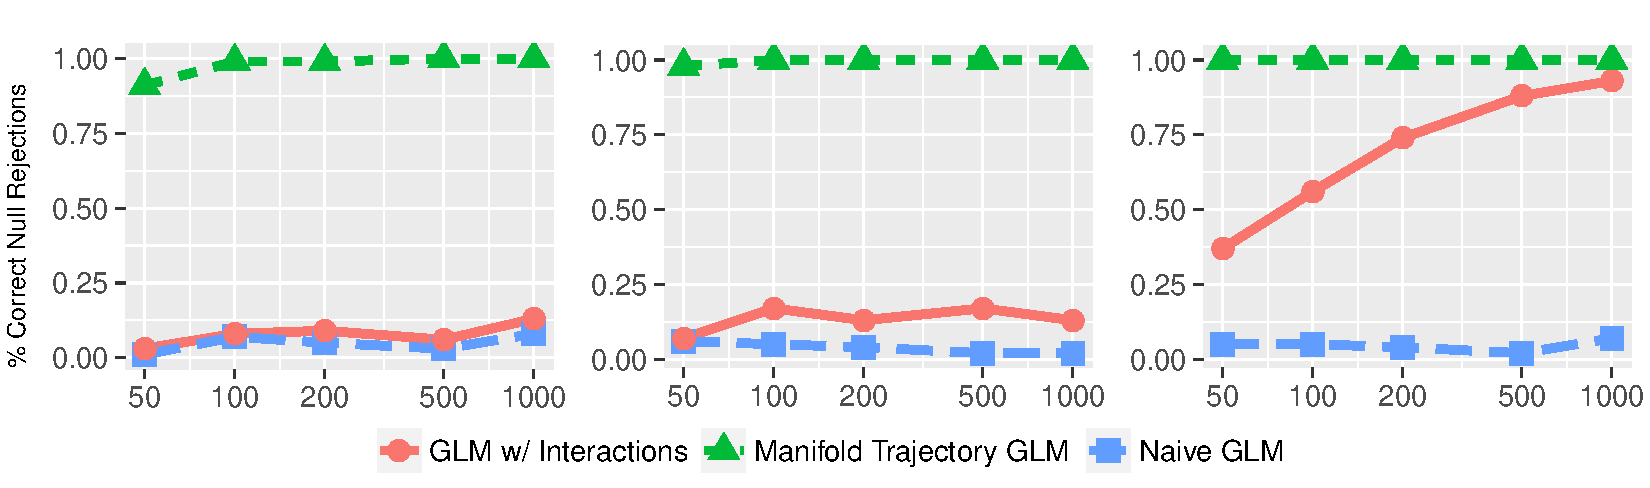
\includegraphics[width=\textwidth]{3_covtraj/figs/sim_results.pdf}
		\caption[Synthetic hypothesis testing true positive rates]{\label{fg:sim_graphs}Correct null hypothesis rejections over 100 runs for three models. For $p = 50$ features, each plot shows the rejection rate
		for $p_t \in \{4, 8, 20\}$ (from left to right) respectively as a function of the number of sample points.}
	\end{center}
\end{figure}
%	
\begin{table}
	{
		\caption{\label{tab:recover-table} Detection Accuracy of hypothesis test scheme (100 runs).}
		\begin{center}
			{\begin{tabular}{lllll}
					\toprule
					\toprule
					& $p_t = 5$& $p_t = 8$	& $p_t = 10$&  $p_t = 15$ 	\\
					\midrule
					$n=10$	&  0.06  &  0.02  &  0.04  &  0.03 \\
					$n=20$	&  0.75  &  0.75  &  0.53  &  0.29 \\
					$n=50$	&  0.99  &  1.00  &  1.00  &  0.80 \\
					$n=100$	&  1.00  &  1.00  &  1.00  &  0.95 \\
					$n=200$	&  1.00  &  1.00  &  1.00  &  0.98 \\
					$n=1000$&  1.00  &  1.00  &  1.00  &  1.00 \\
					\bottomrule
					\bottomrule
			\end{tabular}}
		\end{center}
	}
\end{table}
Figure \ref{fg:sim_graphs} shows the value of our method over these models. For the interaction GLM case, we randomly select interaction terms to include in the GLM, with size $p_t$ (the ground truth number of variables in the interaction). In this way, we approximate the effect of an oracle specifying to the GLM which terms may describe the underlying interaction. 
We report the fraction of significance tests where a significance threshold 
of $p \leq 0.05$ was found for each model, averaged over 100 runs. 
%Simulated data were generated using the procedure outlined for the simulations above, with more details provided in the Appendix.
We see that our proposed scheme consistently achieves near-perfect results in terms of the percentage of null hypotheses that 
were correctly rejected (i.e., there was a significant group-difference signal). The power of scan statistics on 
graphs is particularly evident in the needle in haystack setting where the true differential signal is small ($p_t \leq 8$)
and the sample size is small to medium. When the sample size is large and $p_t$ is also large, the standard linear model with additional interaction terms starts to approach the statistical performance of our algorithm.

%% \begin{figure}[]
%% 	\begin{center}
%% 		\includegraphics[width=0.9\textwidth]{babynames_result_bad.pdf}
%% 		\caption{\label{fig:babyEX} Baby name orderings over time across boys and girls.}
%% 	\end{center}
%% \end{figure}

\section{Baby Name Trends Over Time}
\label{sec:baby}
In addition to the simulations above, we report results from a simple analysis of 
how male/female baby names evolve over time over the last century. 
The United States Social Security Administration provides a publicly available dataset listing the frequency of the 
top 1000 baby names in each state for the last 106 years.
We evaluate our model in this context to examine which ``sub-group'' of states tend to evolve (or change) in their
``name agreement" (or correlation) over time between boy names and girl names.
Here, rather than calculating a sample covariance
at each timepoint, we calculate a rank correlation matrix instead. 
For example, if two neighboring Gulf Coast states, say Georgia and Alabama, substantially 
agreed on both boys and girls names in the period following the second World War, but gradually this agreement 
declined over time for girls (but not boys), 
we expect that our scan statistics on graphs hypothesis test 
will segment out this differential signal (in slope trends) from the planar graph induced by the states sharing 
a border.
Shown in Figure \ref{fig:usmap} are the regions identified using our method, applied on only the rank correlations for the top 10 names for both genders per state per year. Each highlighted region indicates a sub-group
where their ``trends of correlation (or agreement/disagreement)'' in preferred baby names over the last century 
varies between boys and girls. 
%{\color{red} In Figure \ref{fig:babyEX} we show a snippet of the data from an identified subregion.}
%of states that have varying agreement and disagreement of boys and girls names over the last century.
For states not identified by our model (in gray), we can conclude that
the state-to-state name preference-interactions may have still 
evolved over time but we have insufficient statistical 
evidence to conclude that such trends (slopes) are different between boys and girls. 
%https://github.com/msbarry/babymap/
%may still have a strong trend in terms of how the
%state-to-state name preference-interactions 
%evolve over time but we have insufficient evidence to conclude that such trends are different between boys/girls. 
%tend to follow the trends of neighboring states very closely, regardless of sex. 

\begin{figure}
	\begin{center}
		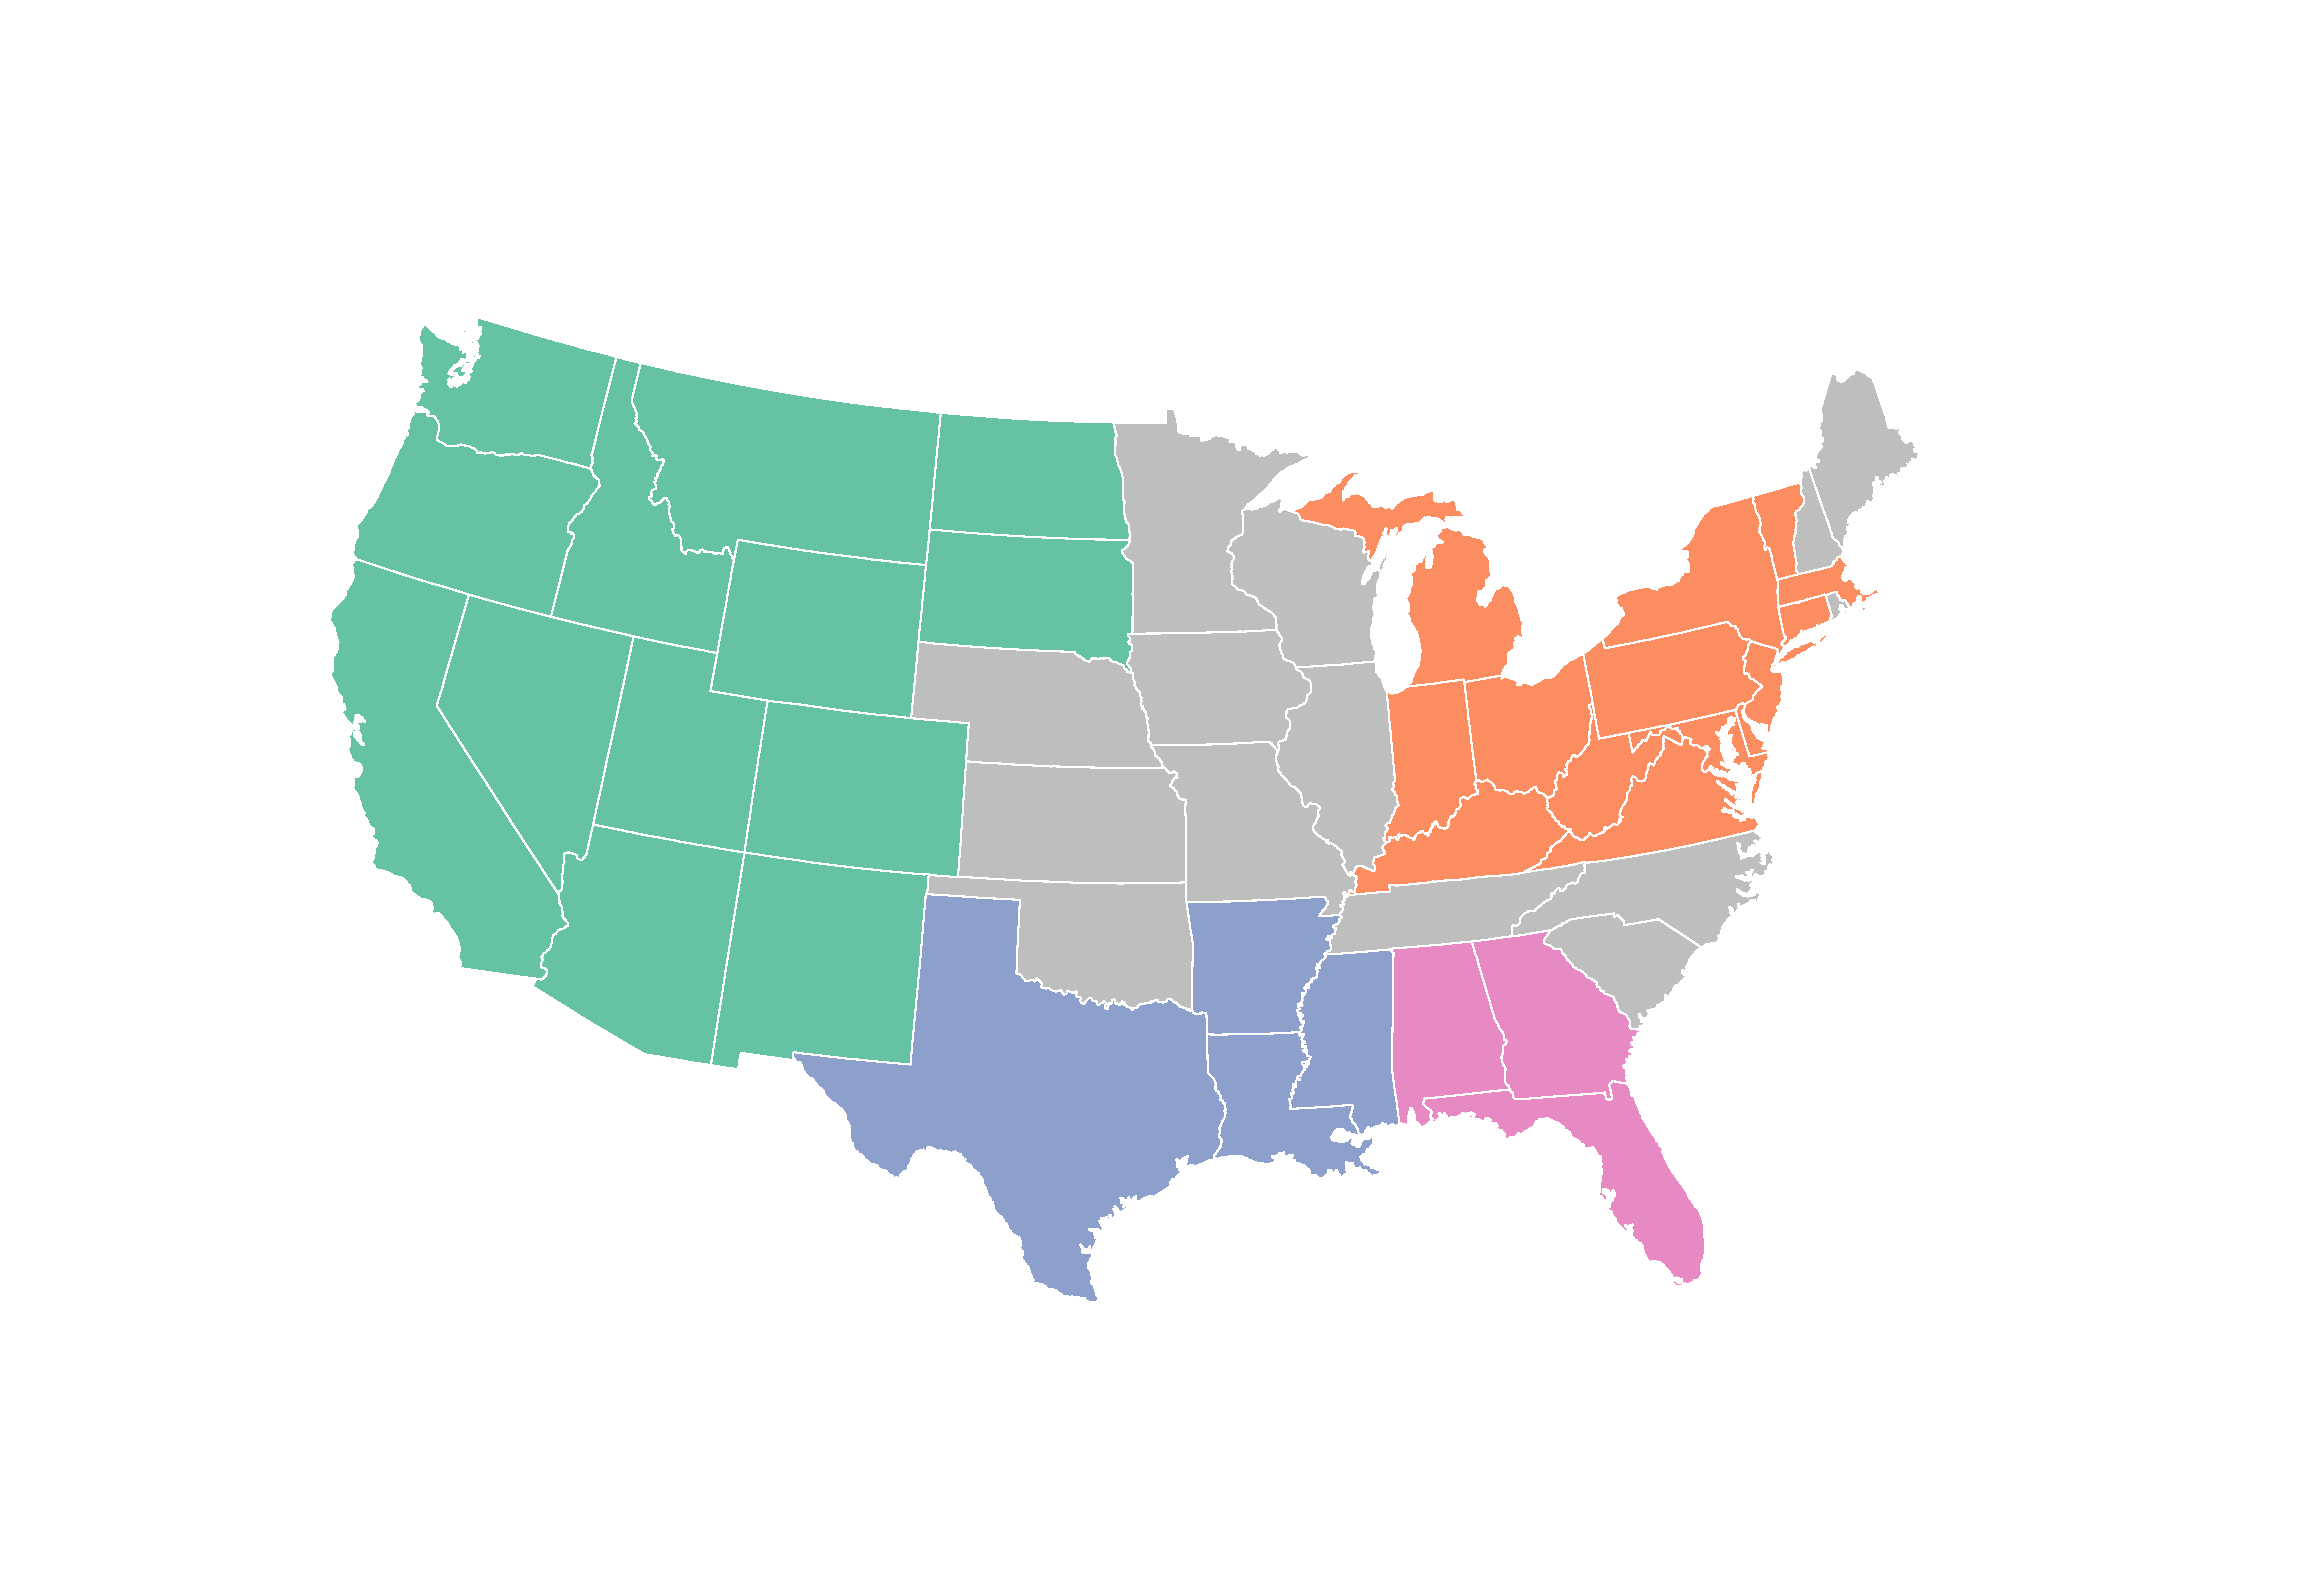
\includegraphics[,trim={5cm 5cm 5cm 5cm}, clip, width=0.7\textwidth]{3_covtraj/figs/babynames_res.eps}
		\caption[Covariance trajectory testing results on baby name frequency.]{\label{fig:usmap} Contiguous states identified as having significantly different time-varying co-occurrences between boys and girls baby names from 1910 to 2015. Best viewed in color.}
	\end{center}
\end{figure}
\section{Identifying Differentially Covarying Features in Preclinical Alzheimer's Disease}
\label{sec:wrap}
% Emacs, this is -*-latex-*-
We now describe experiments and results focused on the key motivation of this work --- to facilitate 
analysis of a longitudinal study of individuals at risk for Alzheimer's disease (AD) where the statistical 
signal is weak (with small to medium sample sizes). We describe the dataset details followed by the analysis and then interpret our conclusions 
in the context of scientific results that have been published in the literature in aging and dementia.

%\subsection{Background}
\paragraph{Study background.} We analyzed data from a 
%unique  neuroimaging obtained through the Wisconsin Registry for Alzheimer's Prevention (WRAP), 
cohort of individuals who have been longitudinally tracked for at least three visits over multiple years, as part of an ongoing study (since 2001)
to understand the disease processes in the brain {\em before} an individual exhibits signs of 
cognitive decline due to Alzheimer's Disease (AD) \citep{sager2005middle}. The study, Wisconsin Registry for 
Alzheimer's Prevention (WRAP)  
is among the largest of its kind in existence, focused on ``preclinical'' AD, i.e., when the 
individuals are still cognitively healthy, offering a window into the early disease processes 
where treatments, drugs and interventions are likely to be most effective. 
%Many participants in this study have been longitudinally tracked for over ten years 
WRAP and its ancillary studies 
acquire neuroimaging data (MRI, PET with different tracers, diffusion MRI) and various clinical test scores, 
genetic and demographic data as well as clinical measures such as Cerebrospinal Fluid (CSF). Our analysis 
seeks to understand subtle group-wise differences in longitudinal patterns of dependencies between these measures at this early stage of the disease. 

\paragraph{Dataset.} The dataset consisted of 114 subjects with imaging data from at least two types of imaging modalities: Positron emission tomography and 
diffusion weighted Magnetic Resonance (MR) images. 
Positron emission tomography (PET) images were used to calculate, using well-validated pre-processing pipelines, 
the mean amyloid-plaque load (an important biomarker for AD) in 16 different anatomical regions of interest in the brain. 
Amyloid plaque is known to be an AD-related pathology and generally {\em precedes} onset of cognitive symptoms. 
Separately, diffusion tensor MR imaging (DTI) data were processed and used to calculate both Fractional Anisotropy (FA) and Mean Diffusivity (MD) in 48 distinct regions \citep{mori2008stereotaxic}. 
DTI images provide information about structural connectivity between gray matter regions in the brain. 
In addition to these $108$ ($48 \times 2 + 16$) image-derived features, 
we also included in the analysis the participant's scores on a battery of cognitive tests, known to be correlated with various neuropsychological functions \citep{lezak2004neuropsychological}. 
%One of the focus of of pre-clinical AD research is to identify biomarkers which may be reasonable indicators of developing pathology. 
%Identifying cognitive and neuroimaging measures that are significant differential trajectories could help in finding these biomarkers. 
%To detect group differences, grouping was performed using subject age, binned into three quantiles. 
Differences were evaluated on various groupings of the subjects which were, for the most part, 
based on known results in the literature.   
Specifically, gender, APOE (Apolipoprotein E) genotype and amyloid positivity (based on thresholding the amyloid plaque summaries) have 
all been evaluated as significant in
AD studies \citep{racine2014associations} but often such analyses involve a population covering a broader disease spectrum where 
the signal is much stronger. 
%Our cohort is still pre-sympotomatic.
%

\paragraph{Is analysis of second order statistics necessary?} In Figure \ref{fig:imagehists}, we present histograms detailing the distribution of two critical cognitive tests, stratified across various groups of scientific interest. Evaluating these distributions were the key motivation for our exploration into the methods described in the paper. Small differences in means across groups {\em regardless of grouping selection (i.e., stratification variable)}, and the saturation that occurs at the ceiling of cognitive test scores and other preliminary experiments conducted by us suggest that standard analyses are not sensitive enough to identify subtle higher-order differences.
\begin{figure}
	\centering
	%\includegraphics[width=0.49\textwidth]{BNTHists.pdf}
	%\includegraphics[width=0.49\textwidth]{TTOTALHists.pdf}
	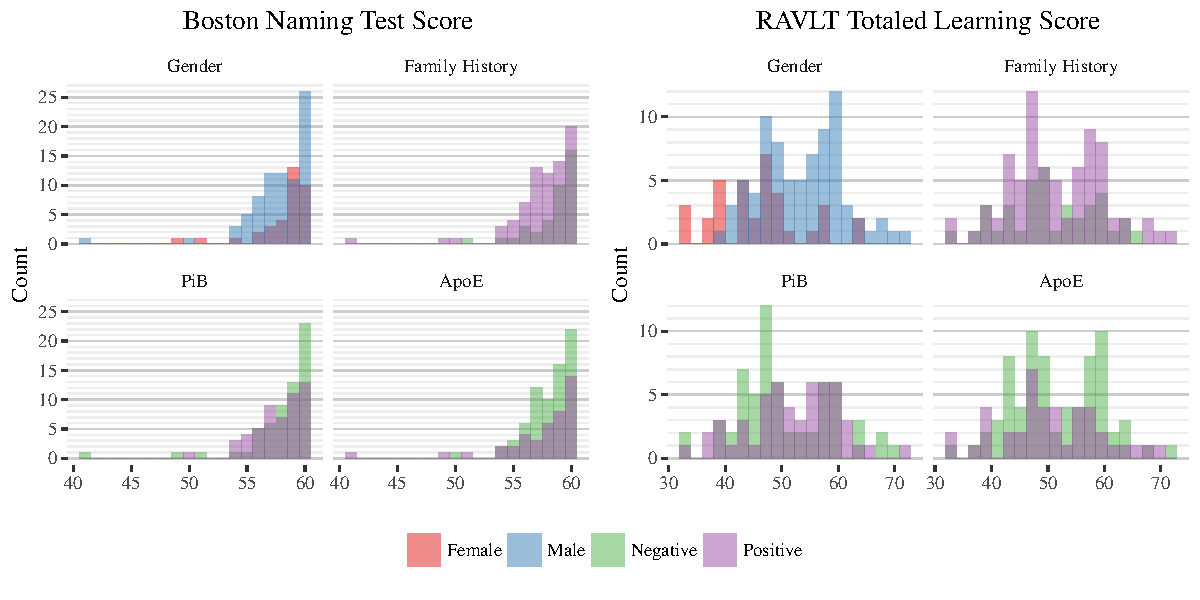
\includegraphics[width=\textwidth]{3_covtraj/figs/hists.pdf}
	\caption[Summary histograms of neuropsychological test scores for preclinical AD participants]{Histograms of the Boston Naming Test Scores and RAVLT Total Scores for all time points for the $114$ individual measurements across different group separations. The means for each test score is not significantly different across different stratification variable.}
	\label{fig:imagehists}
\end{figure}
\subsection{Results for Group difference analysis for individuals with imaging data}
We now describe, one by one, the components of the largest feature subset discovered for each stratification scheme 
and highlight the main scientific findings. In most cases, we provide a brief scientific interpretation of the results
for the interested reader. 
Additional details and results are available in the appendix.
%, along with a longer description of our experimental setup and the covariate models learned for the significant groups.
%

\paragraph{A) Graph Scan Statistics on slope differences across gender.} 
The most significant (based on region-score) subset identified by the gender grouping was between the FA DTI measurement in the left cingulum gyrus 
as well as the scores on the Rey Auditory Verbal Learning Test (RAVLT). In recent AD research, gender has been identified as a factor in the progression 
of various pathology measures (e.g., incidence and prevalence of AD is higher in women \citep{fratiglioni1991prevalence,rimol2010sex}), and has contributed to a formal NIH notice (NOT-OD-15-102). However, we note that previous work in the field has \textit{not} identified gender-related 
differences when looking {\em only} at diffusion measures in the cingulum \citep{lin2014cingulum}. Our algorithm 
successfully identified longitudinal 
changes in {\em interaction} between these variables which supports the earlier results, and provides some evidence that as men and women age, 
their cognitive decline as measured by RAVLT manifests differently in relation to the cingulum gyrus.
%

\begin{table}
	\centering
	\begin{tabular}[t]{ll}
		\toprule
		\multicolumn{2}{c}{\textbf{Gender}}\\ \midrule \midrule
		
		Set 1     & RAVLT Total (1-5) \\ & FA Cingulum  L	\\
		\midrule
		Set 2 & FA Medial lemniscus L	\\ & FA Cingulum (hippocampus) L		\\
		& FA Post thalamic radiation L \\ \midrule
		Set 3    & FA Corticospinal tract R \\ & FA Superior O.F. fasciculus  R \\	\midrule\bottomrule
	\end{tabular}
	\hfill
	\begin{tabular}[t]{ll}
		\toprule
		\multicolumn{2}{c}{\textbf{Genotype: APOE4}}\\ \midrule \midrule
		Digit Span Backward Raw Score & Stroop Color-word Score \\ 
		PiB Cingulum Post L &    PiB Cingulum Post R         \\
		PiB Frontal Med Orb L & 		PiB Frontal Med Orb R \\ 
		PiB Precuneus L & PiB Precuneus R \\ 
		PiB SupraMarginal &  PiB Temporal Mid R \\ \midrule		 \bottomrule
	\end{tabular}
	\caption[Group differences identified across gender and genotype]{\label{tab:wrapIMG}Group difference across Gender (left) and Genotype APOE4 expression (right). Three disjoint sets of features were identified as coavarying significantly differently among gender, while one larger set was identified in the genotype stratification.}
\end{table}


\paragraph{B) Graph Scan Statistics on slope differences across genotype.} 
Next, we stratified the cohort
 based on the genotype known to be most closely linked with AD, i.e., the APOE (Apolipoprotein E) gene \citep{corder1993gene} --- 
we inherit one APOE allele from each parent; having one or two copies of the e4 allele increases a person's risk of getting AD 
whereas the rarer e2 allele is associated with a lower risk of AD. 
Using this stratification, we obtain a low-risk and an at-risk group of individuals. 
Here, we identified amyloid-load regions within the medial and lateral parietal lobes 
%with scores on the Controlled Oral Word Association fluency test \cite{abc}. The temporal gyrus is known to be stimulated when accessing word meaning while reading. Among the group without 
%this specific genotype risk allele, we 
and find that in the ``low-risk" group, the covariances between Digit Span and Stroop Color-Word scores 
(attention and concentration scores) and amyloid load moves from strongly negative towards $0$ as a function of age (Table \ref{tab:wrapIMG}). 
In the ``at-risk'' group 
(APOE4), however, we find that as a function of age, the features become more and more positively correlated. 
Existing studies have shown that the accumulation 
of amyloid is significantly different across APOE4 gene expression \citep{mormino2014amyloid}, and our results provide some evidence 
that the expression of the genotype may interact with cognitive scores as well, {\em even at this early stage of the disease}, 
when the individuals in our cohort are 
cognitively healthy. The sets of features showing a differential signal are presented in Table \ref{tab:wrapIMG}.
%has a real impact on the way in which one might solve language problems. (this sounds odd/needs elaboration)
%

\begin{table}
	\centering
	\begin{tabular}{lll}
		\toprule
		\multicolumn{3}{c}{\textbf{Amyloid Load (PiB Positivity)}}\\ \midrule \midrule
		%		    \multicolumn{3}{c}{Gender}}                   \\\
		Set 1 & PiB Angular L/R & PiB Cingulum Ant L/R \\
		& PiB Cingulum Post L/R & PiB Frontal Med Orb L/R \\
		& PiB Precuneus L/R & PiB Temporal Sup L/R \\
		& PiB Temporal Mid L/R & \textbf{PiB SupraMarginal L} \\
		\midrule
		Set 2     & FA Cerebral peduncle R   & FA Cerebral peduncle L	\\
		& MD Corticospinal tract R	& MD Corticospinal tract L		\\
		& Trail-Making Test Part A Score  & MD Cerebral peduncle R \\ 
		&PET Cingulum Post R  &  \\ \midrule\bottomrule
	\end{tabular}
	\caption{Group difference across Amyloid Load (PiB Positivity)}
	\label{tab:wrapPIB}
\end{table}

\paragraph{C) Graph Scan Statistics on slope differences across amyloid load positivity.} 
As briefly described above, amyloid load is an important biomarker for AD. For our analysis, amyloid (or PiB) positivity 
is calculated using the mean amyloid PiB measures across all brain regions using a PiB PET image scan of the participant. 
When we used this measure for stratification (threshold was set at $1.18$, following \cite{darst2017pathway}), 
our model identified fifteen of the sixteen PiB regions that were input to the model when the density of the oracle graph was set to be high. 
This result is as expected, but interestingly we find that controlling for the linear combination of the features (through centering), 
the residual error \textit{still} has significant signal with the PiB positivity measure, indicating that amyloid burden \textit{interactions} 
across brain regions plays a very important role in AD progression \citep{hardy2002amyloid,hardy1992alzheimer,tanzi2005twenty,jack2010brain}. When the sparsity of the oracle graph was increased, however, four neighboring regions, the left and right corticospinal tract and the left and right cerebral peduncle were identified on both PiB and DTI measures (supported by the literature \citep{douaud2011dti}), together with Part A of the Trail Making Test (see Table \ref{tab:wrapPIB}) which 
happens to be used in AD diagnosis \citep{albert2011diagnosis}. 
This suggests that changes in atrophy within these regions, as measured by DTI, co-occur with changes in amyloid burden. Additionally, because these regions are highly correlated with rough and fine motor ability \citep{naidich2009duvernoy}, it seems plausible that amyloid positivity will lead to higher `covariation' in the regions associated with 
a measure of fine motor speed, i.e., the Trail Making Test.

\subsection{Results for for Group difference analysis for individuals with Cognitive Testing data}

In addition to the dataset presented above, we apply our method to a much larger dataset consisting of approximately 1500 individuals with only cognitive testing data collected in a longitudinal manner. Each individual was administered these tests for between two and three time-points, yielding approximately $n = 4000$ samples for our model. For each assessment, a conference of experts applied a diagnostic label indicating normal cognition or mild cognitive impairment. Using this binary classification, we can stratify our population for group difference analysis.
We find that among many different significant subsets, the covariance trajectory among the scores on both parts of the Trail-Making Test and 
on all trials of the RAVLT test explain a significant group difference. These have previously been shown to be the {\em most sensitive tests} for 
early cognitive decline \citep{albert2001preclinical}. 
Table \ref{tab:wrapCC} displays the other tests identified by our algorithm, and additional experiments on this larger cohort 
can be found in the appendix. 
%

\begin{table}
	\centering
	\begin{tabular}{ll}
		\toprule
		\multicolumn{2}{c}{\textbf{Expert Consensus Diagnosis}}\\ \midrule \midrule
		WAIS-3 LNS Raw Score &
		Boston Naming Test Total Score \\
		RAVLT A2 Raw Score &
		RAVLT A3 Raw Score \\
		RAVLT A4 Raw Score &
		RAVLT A5 Raw Score \\
		RAVLT A6 Raw Score &
		RAVLT Delayed Recall Raw Score \\
		Trail-Making Test Part A &
		Trail-Making Test Part B \\
		Clock Drawing Test Score &
		CES Depression Scale Score \\
		\bottomrule
		\bottomrule
	\end{tabular}
	\caption[Localized results across expert clinical diagnosis]{Group difference localization across expert clinical diagnosis. With significantly more samples and a larger set of cognitive tests, those above were identified as significantly different across the expert consensus measure.}
	\label{tab:wrapCC}
\end{table}

\subsection{Baseline.}

In various experiments on this dataset, when the MMGLM procedure is performed for the entire feature set in totality ({\em not} 
utilizing any of the proposed ideas based on scan statistics), 
and the null distribution derived using permutation testing, the procedure {\em yields no significance across \textit{any} 
scientifically interesting group stratifications}. 
This implies that the ability to search over different blocks of the covariance matrix is critical in identifying meaningful group differences 
in the trajectories, unavailable 
using alternate schemes. For instance, simpler strategies work well enough for datasets such as ADNI -- 
  which includes diseased subjects as well as controls -- 
  where the signal is stronger and even temporal modeling may be unnecessary.
  While the scientific results need to be interpreted with caution and reproducibility experiments on 
other similar datasets (both within the US and internationally) are in the planning phase, 
we believe that the ability to localize 
differences in these interaction patterns in a statistically rigorous manner is valuable and these findings can be investigated standalone, via 
more classical schemes (e.g., structural equation modeling). 



\section{Conclusions}
The analysis of datasets to identify where clinically disparate groups differ is pervasive in biology, neuroscience, genomics and epidemiological studies. 
We find that graphical models are an ideal tool to analyze high-dimensional data in these areas but have been sparingly used for the analysis of 
group-wise differences, especially in a longitudinal setting. 
Motivated by an application related to longitudinal analysis of imaging and clinical/cognitive data from otherwise healthy individuals 
who are at risk for Alzheimer's disease (AD), we show how a combination of manifold regression with a generalization of scan statistics to the graph setting yields 
tools that can be directly deployed. 
We present an efficient algorithm and develop the theoretical results showing the regimes where its application is appropriate. 
In various experiments, while the standard schemes are not sufficiently powered to detect the signal, our proposed formulation is able to 
detect meaningful group difference patterns, many of which have a clear scientific interpretation. 
We believe that these results are promising for the neuroimaging application 
described and other regimes where group-wise analysis is desired but the number of features is large. 
We will revisit work in this chapter in some follow-up work, described in Chapter~\ref{chap:discuss}.
\todo{ch3: reference other work (ISBI/TMI) here or in last chapter?}
\todo{make a public repo with the code without medinfo}
